\documentclass[12pt]{article}  % [12pt] option for the benefit of aging markers
\usepackage{amssymb,amsthm}    % amssymb package contains more mathematical symbols
\usepackage{graphicx}          % graphicx package enables you to paste in graphics
\usepackage[capposition=top]{floatrow}
\usepackage{setspace}
\usepackage{float}
\usepackage[backend=bibtex,sorting=nyt,firstinits=true]{biblatex}
\usepackage{hyperref}
\usepackage{longtable}
\usepackage{wrapfig}
\usepackage[titletoc,title]{appendix}
\usepackage{pdfpages}
\usepackage{color, colortbl}
\usepackage{tikz}
\usepackage{pgf-pie}
\usepackage{pgfplots}
\usepackage{subcaption}
\usepackage{mathdots}


\usepackage{lipsum}
\usepackage[margin=2cm]{geometry}

\definecolor{Gray}{gray}{0.9}

\definecolor{Green}{RGB}{0, 153, 0}
\definecolor{Yellow}{RGB}{255, 255, 51}
\definecolor{Red}{RGB}{203, 0, 0}

\definecolor{lightgray}{rgb}{.9,.9,.9}
\definecolor{darkgray}{rgb}{.4,.4,.4}
\definecolor{purple}{rgb}{0.65, 0.12, 0.82}


\addbibresource{references.bib}
\newcommand{\rid}[1]{\centering #1-\ifnum\value{requirement}<10 0\fi\arabic{requirement}
\stepcounter{requirement}}
\newcommand{\tag}[1]{\textless {#1}\textgreater}





%PHP Code Listings Code %

\usepackage{listings,xcolor}
%\usepackage{inconsolata}

\definecolor{dkgreen}{rgb}{0,.6,0}
\definecolor{dkblue}{rgb}{0,0,.6}
\definecolor{dkyellow}{cmyk}{0,0,.8,.3}
\definecolor{backcolour}{rgb}{0.95,0.95,0.92}

\newcommand{\phplisting}{\lstset{
  language        = php,
  basicstyle      = \footnotesize\ttfamily,
  keywordstyle    = \color{blue},
  stringstyle     = \color{red},
  identifierstyle = \color{black},
  commentstyle    = \color{gray},
  emph            =[1]{php},
  emphstyle       =[1]\color{darkgray},
  emph            =[2]{if,and,or,else},
  emphstyle       =[2]\color{darkgray},
  numbers = left,
  backgroundcolor=\color{lightgray},
  frame = single, 
  framexleftmargin=1.5em,
  xleftmargin=2.5em,
  breaklines= true,
  showstringspaces=false,
  escapeinside={(*@}{@*)}
  }}
  
%End of PHP Code Listings Code %


\lstdefinelanguage{JavaScript}{
  keywords={typeof, new, true, false, catch, function, return, null, catch, switch, var, if, in, while, do, else, case, break},
  keywordstyle=\color{blue}\bfseries,
  ndkeywords={class, export, boolean, throw, implements, import, this},
  ndkeywordstyle=\color{darkgray}\bfseries,
  identifierstyle=\color{black},
  sensitive=false,
  comment=[l]{//},
  morecomment=[s]{/*}{*/},
  commentstyle=\color{gray}\ttfamily,
  stringstyle=\color{red}\ttfamily,
  morestring=[b]',
  morestring=[b]"
}

\newcommand{\jslisting}{
\lstset{
   language=JavaScript,
   backgroundcolor=\color{lightgray},
   extendedchars=true,
   basicstyle=\footnotesize\ttfamily,
   showstringspaces=false,
   showspaces=false,
   numbers=left,
   numberstyle=\footnotesize,
   numbersep=9pt,
   tabsize=2,
   breaklines=true,
   showtabs=false,
   captionpos=b
}}


%%%%%%%%%%%%%%%%%%%%%%%%%%%%%%%%%%%%%%%%%
%										%
%     			Title					%
%										%
%%%%%%%%%%%%%%%%%%%%%%%%%%%%%%%%%%%%%%%%%
\title{Digital Lab Marking System \\~\\  \large{Heriot-Watt University} \\~\\ Deliverable 1: Final Year Dissertation \\~\\ MEng Software Engineering}
\author{Lewis Francis McNeill\\
supervised by
Peter J King}

\begin{document}
\maketitle
\pagenumbering{gobble}



%%%%%%%%%%%%%%%%%%%%%%%%%%%%%%%%%%%%%%%%%
%										%
%     		    Declaration				%
%										%
%%%%%%%%%%%%%%%%%%%%%%%%%%%%%%%%%%%%%%%%%
\newpage
\setcounter{page}{1}
\pagenumbering{roman}
\doublespacing
\textbf{\Large{Declaration}} \\[2em]
I, Lewis Francis McNeill, confirm that this work submitted for assessment is my own and is expressed in my own words. Any references, made within it, of the works of other authors in any way (e.g., ideas, equations, figures, text, tables, programs) are properly acknowledged at any point of their use. A list of the references employed is included.
\\
\\
Signed: Lewis McNeill
\\
Date: \today


%%%%%%%%%%%%%%%%%%%%%%%%%%%%%%%%%%%%%%%%%
%										%
%     		    Abstract				%
%										%
%%%%%%%%%%%%%%%%%%%%%%%%%%%%%%%%%%%%%%%%%
\newpage               
\begin{abstract}
\noindent
The aim of this dissertation project is to replace the current system for the marking of computer labs with a new digital system. This will enable lecturers to create a marking scheme online. Lab helpers will select the student they are marking and the marking scheme will then be loaded, marks will be entered and then made immediately available to both student and lecturers to view. It will also provide useful statistics for both student and lecturers.
\end{abstract}
\newpage 

\tableofcontents
\newpage
\listoffigures
\listoftables
\lstlistoflistings


%%%%%%%%%%%%%%%%%%%%%%%%%%%%%%%%%%%%%%%%%
%										%
%     		Introduction				%
%										%
%%%%%%%%%%%%%%%%%%%%%%%%%%%%%%%%%%%%%%%%%
\newpage   
\setcounter{page}{1}
\pagenumbering{arabic}
\section{Introduction}

The current system for marking of computing science labs is to use multiple lab helpers, each given a list of students and the marking scheme for them. Generally marking schemes consist of a selection of tasks which students must have completed and lab helpers tick them off when this has been achieved. The biggest problem with this part of the marking is the length of time it takes lab helpers to locate the students on the list. This causes frustration with increased waiting times for students.  Multiple other issues  can also  arise from this: students can be marked by two helpers and obtain different grades from both; the lab helper omits to  tick off a completed task; they assign  marks for the wrong student on the sheet or simply they misplace the actual marking sheet.

After the lab helpers have completed their marking, the sheets are provided to the lecturer who collates them into one spreadsheet to calculate the marks. After that it is entered it into vision. This too can cause its own set of problems-the chances of transcription errors are increased as it is possible for the lecturer to misread marks when they are transferring them across. The lecturer may not enter the marks immediately into the spreadsheet increasing the chance that a marking sheet goes missing, and finally this system means that students are having to wait even longer to receive their results.

The objective is to develop a system that will reduce and hopefully eliminate the problems of the current system. Along with this, it should hopefully reduce the amount of time taken to mark students’ work and therefore speed up labs in general. It should also enable students to see their grades immediately, allow lecturers to see the result of the assignments as they are being marked and make marking quicker for lab helpers.




\newpage
\section{Aims and Objectives}
\subsection{Aim}
The aim of this dissertation is to design and implement a system for the digital marking and analysis of computer labs and to help improve the speed at which they are marked. The system will also provide useful statistics for both lecturers and students.

\subsection{Objectives}
\label{section:object}
\begin{itemize}
\item Simplify the way that labs marks are currently processed.
\item Allow lecturers to create marking schemes on-line that lab helpers can access. 
\item Lab helpers can mark students in labs using marking schemes.
\item Lab helpers able  to mark labs using an on-line application.
\item Allow students to see the mark they achieved from the lab instantly.
\item Provide useful statistics and graphs for lecturers and students.
\item Provide different views for student, lab helpers and lecturer.
\end{itemize}



\subsection{Scope}





%%%%%%%%%%%%%%%%%%%%%%%%%%%%%%%%%%%%%%%%%
%										%
%     	   Literature Review			%
%										%
%%%%%%%%%%%%%%%%%%%%%%%%%%%%%%%%%%%%%%%%%
\newpage
\section{Background Information}
This section contains summaries of literature relating to the topic and should help to create a context for the development of a digital marking system. It will cover which marking systems are currently used, also which current digital marking systems actually exist and why they are an improvement. Along with this it will also cover how to control what users are allowed to see, as well as explaining systems for creation of custom website forms, and finally it will cover the graphical displaying of statistics. 


\subsection{Web Applications}

The digital lab marking system will be developed as a web application. To help understand how web applications are built this sub section covers the core technologies required to develop web applications.

\subsubsection{HTML}
HTML is short for Hypertext Markup Language and is a markup language which in fact is less a programming language and more a set of instructions \cite{brooks_introduction_2007}. It creates the structure of a website through the use of elements which are represented by: example tags include:\tag{html}, \tag{href}, \tag{a}. 

\noindent An individual element is made up of an open tag (\tag{a}) and a closing tag which is the same as the opening tag but includes a back slash at the start (\tag{$\backslash$a}). Elements can exist inside other elements creating a hierarchical structure.

\noindent Web browsers do not display the elements and tags directly \cite{w3_introduction_nodate} but instead they process these elements to decide how the web page should look and then renders it in the browser's screen for the user to interact with. The downside to web browsers deciding how to render elements is that different browsers can choose to render the same element two different ways. For instance if a web page was loaded using Google Chrome it may render a table where the column width is not defined with each column getting equal space, but if the same table was loaded using Fire-fox it may decide that each column only gets the minimum size required and therefore the table looks narrower. This can have a really major effect if the the website was designed with accurate measurements in one browser and another calculates sizes differently resulting in the website displaying wrongly.    


\subsubsection{Cascading Style Sheets}
Cascading Style sheets (CSS)\cite{lie_cascading_2005} are used to change the properties of elements created using HTML; through the changing of these properties developers can change the look and response of a website. Developers can also create classes and ids, both of which are given names and then element properties are set inside. This means for instance a class called "bigText", which makes the text large and bold- when a element uses this class all the specified properties are changed. HTML elements can have multiple classes but can only have one id which creates a priority system. 

The priority system \cite{noauthor_cascading_nodate} is where the cascading part of the style comes into effect, elements inherit the property of any class assigned to them, but if another class is added it cascades through the current set properties changing any that the class also declares. This means that classes declared later have a higher priority for example class=" bigText smallText", in this the element has a big and small text class. Since the smallText class is declared after bigText the elements properties will set to it. The only thing that would not have changed are properties declared by the id, since an element can only have one id it has a higher priority than any class and so will override properties with its own values.  

This priority and cascading system also works with multiple files. If two css files are being used by an HTML document and both declare a class called "bigText", then the "bigText" class from the css file that is declared last, will be the one that is used. This will be very useful for this project as it allows for the use of frameworks which will provide their own css files, but adding my own file afterwards will allow me to customise the initial css file.

As part of this project I will be using CSS 3 which at time of writing (2017) is the currently agreed standard \cite{noauthor_css_nodate}.


\subsubsection{JavaScript}

JavaScript is a high-level interpreted language and loosely typed, meaning that you do not need to declare the type of  variable. JavaScript programs are called scripts and can interact with the user, their web browser, and is capable of editing HTML content that is displayed inside the user's browser \cite{flanagan_javascript:_2006}. JavaScript is generally embedded into HTML web pages and is usually called client-side JavaScript as the scripts are run on the user's computer not the web page's server.



\subsubsection{PHP}
\label{sec:php}

PHP stands for Hypertext Preprocessor and is an open source scripting language first developed in 1994 \cite{noauthor_php:_nodate} which can be embedded into HTML. Unlike HTML which is sent to the user and processed by their computer, PHP scripts are instead processed by the website server. Once it has been processed HTML is generated and sent to the user. 

PHP currently has two major versions which are version 5 and 7. For this project I will be using version 5.6.25 as version 5 is still the most common version of PHP \cite{noauthor_usage_nodate} with 95\% of websites that use PHP using version 5. It also allows for easy installation of the lab marking system into the university's server.



\subsection{Marking Systems}

\subsubsection{Lecturer Based}
The way lecturer based marking works is that students complete their assignment, the lecturer or tutor marks it and provides results in a timely manner with useful feedback which can be majorly important in helping students improve their skills  \cite{tang_investigating_2011}.

The advantage of this style of marking is that students can obtain useful feedback from their lecturer that can help improve their learning.  An article study \cite{higgins_conscientious_2002} found that of the students, when surveyed 82\% agreed to the question "I pay close attention to the comments I get" in response to assignment feedback.

A downside to this style of marking is that as the number of students increases on courses the amount of time required to mark assignments consequently takes longer and in some cases this can actually cause marked assessments to be scrapped completely due to the amount of time taken to give feedback to students \cite{brown_assessment_1999}.


\subsubsection{Peer Based}
To cope with increasing class sizes some courses are beginning to move towards peer marking. Peer marking system works by having students assess each other and in some cases  the students produced their own marking criteria \cite{orsmond_use_2000}.

This style allows  students to gain experience in evaluating other people's work, which some graduates feel is a necessary skill to possess. \cite{langan_insights_nodate}. Peer marking also deals with increasing amounts of students very well- this is because as the number of students increases the number of markers also increases!

Peer marking however has its own set of problems - for example, "Students may have a less well developed sense of the criteria compared to the lecturer which could lead to a lack of reliability of student marking." \cite{orsmond_use_2000}.



\subsection{Digital Marking Systems}

\subsubsection{Reasons for Digital Marking}
Digital marking systems are designed to mirror the current paper based marking systems but with the advantage of the electronic environment \cite{heinrich_online_2003}. These systems help to reduce the increasing workload caused by more and more students taking courses. Along with this it also allows administrative tasks associated with coursework to be automated, thus enabling more time for other tasks.\cite{joy_effective_1998}.

For students digital marking is great as it allows for quick feedback as the assessor is able provide students with feedback immediately after they have written it up, instead of having to wait for a class to receive it. In one study\cite{dahl_turnitin_2007} they found that 78\% of students would like get their feedback  electronically .

According to the highlighted article \cite{derby_duplication_2008} plagiarism is on the rise amongst student. This is where digital marking can help to reduce plagiarism as the programme can  do what a human marker cannot. They can compare a submission with thousands of documents and judge if a person has plagiarised. They can also help to show patterns in assignments and marks that normally might go unnoticed.

\subsubsection{TurnItIn}
There currently exists an on-line electronic plagiarism system called TurnItIn, \cite{noauthor_turnitin_nodate} currently being used by many universities around the world. It allows students to upload their essay assignments online. It then checks for plagiarism in the document by searching the internet and using a large database of documents. After it processes the document it assigns a plagiarism percentage and highlights any areas that were plagiarised. Lecturers can then login and view all the submitted documents and mark them .\\
Current research highlighted \cite{dahl_turnitin_2007} conducted a questionnaire and found that students felt that the system was easy to use and more convenient than having to provide paper copies. It also found that 50\% of students strongly agreed and 33.3\% just agreed that they preferred to have their grade shown online rather than have a cover sheet.

\subsubsection{BOSS System}
The BOSS system  was developed at the University of Warwick to help deal with their problem of having too many students for the number of staff and yet wanting students to have accurate and quickly available feedback \cite{joy_boss_2005}.
It is an electronic submission and assessment system created to allow computing science students to submit their programming assignments and have them tested and marked online \cite{joy_effective_1998}. The system is not designed to remove human markers completely, instead simply "assist the instructor in achieving a quicker, more accurate and more consistent assessment of programming assignment"\cite{joy_boss_2005}.

When a file is first submitted it is run through a plagiarism check to make sure that the submission is actually the student’s own work. It also checks that the submission passes pre-set tests to make sure it works. After this it goes into the evaluations stage, since evaluation attributes of code can be very subjective what the second step does is generate metrics about the submitted program. Some of these metrics are a number of comments and percentage of methods declared \cite{joy_effective_1998}, which will help human markers evaluate the submission quicker.




\subsubsection{Ceilidh}

The Ceilidh System was developed at Nottingham University, it is described as "a courseware assessment and management system" \cite{benford_ceilidh:_nodate}. It was designed to support teaching and to do so it was required to manage courses, process the assessment of students, support learning and present information to students. The requirement that is of most interest is that of the processing of student assignments.

Ceilidh was to "perform automatic marking of students work in various forms" \cite{benford_ceilidh_1995} these forms included: Computer programs, multiple different types of questionnaires and exercised and finally reports. 

According to the highlighted article \cite{benford_ceilidh_1995} at the time of Ceilidh's development Nottingham University computing classes contained roughly 160 students and required multiple staff and post graduate students to mark all the programming submissions. It would often result in a long time between submission and results being handed out, and the marking standard would vary quite significantly.

This all changed with the creation of Ceilidh, students could submit their code and get a response in few seconds, and with it being a machine it was completely impartial- meaning that there was a uniform marking standard across all the students. As Ceilidh was further developed, lecturers gained more control over which statistics were immediately available to students. The digital system also allowed for easy storage of student submissions, so they could be easily referenced in case of plagiarism, also the centralised storage of student results meant that lecturers saved time by not having to gather up all the marked results from other people. 






\subsection{User Access Views}

\subsubsection{Social Media}
Controlling the view that users have, based on their access level, is common practice. Social media websites for instance allow users to limit what others can see, through the use of a privacy setting \cite{tufekci_can_2008}. This means that another user's view is determined by the access level they are given: for example, a user that is a friend will have a higher access and be allowed to see their whole feed, while another user's access may only allow them see the profile name.

\subsubsection{Database Controlled Access}
The patent highlighted \cite{noauthor_system_1997}, describes a system of limiting user web page access through the use of relation databases. The system would work by using two databases; one would hold a list of all the url's and associated access level, while the second database would hold all the user id's along with their assigned access level. When a user requests a webpage, the access level for that webpage and the user are looked up. If the users do not have the appropriate access they are denied permission to load the page and depending on implementation may be redirected to another webpage.
The design of this system is well suited for scalability since no matter how large the two datasets are only one piece of data is need from each database to confirm whether a user is allowed access.


\subsection{Custom Input Forms}

\subsubsection{SurveyMonkey}
Survey Monkey \cite{finley_surveymonkey_1999} is an example of custom web forms being created by users. Founded by Ryan Finley in 1999 Survey Monkey enables users to create their own surveys and easily distribute them. It builds the surveys by letting the user select the contents of the question and what the response type will be: The user can also decide if the responses are completely anonymous by default and the participants ip address is stored when they complete the survey. The users can continue to add as many questions as they would like, even after the survey is initially created. After designing the survey the user chooses how they would like to have their survey distributed. The available options that can be selected are a web link, social media, email or embeddable on a website \cite{waclawski_how_2012}.

When participants complete the survey their results are immediately stored and the results of the survey are visible to the user by logging into their account on surveymonkey. They can choose to look at the responses individually or look at metrics about how participants responded.


\subsubsection{Customizing Forms In Electronic Mail Systems}
\noindent
A patent \cite{noauthor_customizing_2006} describes a process for user-customisable forms in an e-mail system where the administrator selects custom field types and behaviours.  For example current e-mail forms have

\begin{wrapfigure}[7]{r}{0.5\textwidth}
\vspace*{-\baselineskip}
\begin{figure}[H]
\includegraphics[width=0.7\textwidth]{images/emailform.png}
	\caption{Example Form (Patent \cite{noauthor_customizing_2006})}
	\label{fig:emailform}
\end{figure}
\end{wrapfigure}

\noindent
a field for address, subject and one for the the actual message to be sent. While an example of what the patent is suggesting can be seen in figure \ref{fig:emailform}, it shows the inclusion of additional fields allowing for wide variety of form to be created and not limit the users to  the few forms that already are designed.\\
This increased flexibility in email forms would allow for easier  interpretation of messages, making responding or providing information via email a lot simpler and quicker.


\subsection{Development Tools}

As part of this developing the lab marking system there will be a wide variety of different development tools used. To help understand how the system is developed these different tools and how they function are explained here.  



\subsubsection{jQuery} \label{sec:jquery}
jQuery is an open source JavaScript library, that is designed to improve the default Javascript used for web development \cite{jquery.org_jquery_nodate}. It makes it easier to perform many actions such as: event handling, Ajax and animation. jQuery also functions on mobile devices meaning that developers do not have to worry that scripts developed for desktop computers will not function correctly on mobile devices.  

\subsubsection{Ajax}
The way that normal websites function is that the user sends a request to the server, the server then processes the user's requests and then creates and sends a response. Once the the user receives this response the web browser interprets it and displays the web page\cite{smith_simplifying_2006}. This process model causes long periods of delay for users as they have to wait for the server to process their request and then wait for the browser to process the response. Meaning users have very disjointed experiences as they have to wait for the whole page to reload every time they try to navigate through it. This is where Ajax comes in as it provides an improved process model that enhances users' experience.  

 Ajax stands for asynchronous JavaScript and XML \cite{jquery.org_ajax_nodate}. It enables browsers to communicate with servers without needing a web page to reload. Ajax's requests are triggered using javascript, though as stated in the previous section (\ref{sec:jquery}) jQuery made the process of triggering Ajax's requests a great deal easier.  
 
 Ajax is made up of a collection of different technologies but each individual technology can exist on their own \cite{garrett_ajax:_2005}. The technologies that make up Ajax are:
 
 \begin{itemize}
 \item HTML and CSS
 \item Dynamic display and interaction
 \item Asynchronous retrieval of data
 \item Javascript
 \end{itemize}



\subsubsection{Bootstrap}
Bootstrap is a front-end framework \cite{noauthor_bootstrap_nodate} designed to help developers create dynamical responsive websites quickly and easily. It provides cascading style sheets and java-script files which are designed to work on all devices.

The way which bootstrap helps create a dynamically responsive website is through the creation of a grid pattern. It breaks the screen up vertically with 12 equally sized sections calculated by percentage. When elements are created the developer declares how many sections wide the element will be. This means that if the screen is scaled down it will still maintain that percentage of the screen size, so the element will scale larger or smaller. Developers can also set an element to use a different number of sections depending on the size of the screen, which means that if a table is initially given four sections then when the screen squashes the table too much then it can be given more sections and therefore more room to expand.

Bootstrap also provides pre-designed navigation bars, side bars, easily customisable button designs and form designs. Altogether this will help speed up the development of the user interface.

The reason that I am using Bootstrap for this project is that is specifically designed for projects that use mobile devices. This will make is easier to build a desktop and mobile version of the lab marking system meaning more time can be spent of the development application's actual functionality.



\subsubsection{PHP Unit}

PHP Unit is a testing framework for PHP. It is designed to allow the easy creation of automated tests in the form of unit tests \cite{bergmann_phpunit_2005}. 

The most recent stable version is PHPUnit 6.0, this version is only compatible with PHP version 7 and was released on the 8th of February 2017. Since I am using PHP 5.6.25, as stated earlier in Section \ref{sec:php}, I cannot use this most recent version and will instead be be using an older stable version 5.7 which supports PHP version 5.6, 7.0 and 7.1. That version was released on 2nd December 2016.



\subsubsection{D3}
D3 \cite{bostock_d3.js_nodate} is a javascript library, which was designed for the creation of interactive visualisations of data and was first developed in 2011. D3 uses precreated Javascript functions to create scalable vector graphics (SVG's) which are embedded into the HTML of websites."SVG is a language for describing two-dimensional graphics in XML"\cite{ferraiolo_scalable_2000} and can have displays changed  using Cascading Style Sheet (CSS).  \\
Data-sets can also be bound to an SVG allowing for a visual way to interpret the data-set, and as the data-set changes the SVG will be changed allowing for a dynamic display.



\subsubsection{CakePHP}
CakePHP is an open source framework for php. It is developed to help the rapid development of web applications and make them simpler,faster and less complex to build \cite{noauthor_cakephp_nodate}. It allows the development of well structured and robust web applications \cite{plekhanova_evaluating_2009}, and its latest version is version 3.3 called "Red Velvet" which can be downloaded from (https://cakephp.org/).

The usefulness of the framework comes in the form of its predefined functions, which allows for a more secure code, since you cannot accidental forget to escape character from input as the functions automatically do this. Cakephp helps to improve the maintainability of systems as it is easy to understand with plenty of comments.

A downside to cakephp is its testability, compared to other web frameworks it lacks in testing tools and does not contain a testing environment \cite{plekhanova_evaluating_2009}.





%%%%%%%%%%%%%%%%%%%%%%%%%%%%%%%%%%%%%%%%%
%										%
%     		 Requirements				%
%										%
%%%%%%%%%%%%%%%%%%%%%%%%%%%%%%%%%%%%%%%%%
\newpage
\section{Requirements}\label{section:require}
\newcounter{requirement} \stepcounter{requirement}


\subsection{Requirements Analysis}
To help discover the requirements of the lab marking system I created a requirements analysis questionnaire(Full questionnaire in Appendix \ref{app:requirements}), the questionnaire was given both to lab helpers and to lecturers to help understand their individual requirements from the system. 

The results of the requirements analysis were used to develop and refine the  list of requirements displayed- functional requirements can be found in section \ref{sec:func} and non-functional requirements in section \ref{sec:non-func}.



\subsection{Requirements}
\label{sec:requirements}
Requirements for the system are each given an id depending on the type of requirement: FR for functional requirements and NFR for non-functional requirements.

Along with this, each requirement has a description stating what the requirement is and a priority is assigned using the MoSCoW prioritization method discussed in the next section (\ref{sec:moscow}).


\subsubsection{MoSCow Prioritisation}
\label{sec:moscow}

MoSCow Prioritisation \cite{noauthor_moscow_2015} was designed to be used in projects that utilise agile development and have a fixed time limit in which to be completed. Its method is that all the requirements of the project are prioritised into four categories, these are:

\begin{itemize}

\item \textbf{Must:} This category of requirements makes up the "\underline{M}inimum \underline{U}sable \underline{S}ubse\underline{T}" of requirements that the project must implement to be successfully delivered.

\item \textbf{Should:} This category contains requirements that are not vital to the delivery of the project, but their absence can affect the project overall. 

\item \textbf{Could:} This category contains requirements that are wanted in the system but are less important than the "should" priority. Reasons that a requirement "would" become a "could" instead of a "should" are if the amount of time taken to implement the requirement and how much of an affect its absence would have on the project.   

\item \textbf{Won't:} This category contains all the requirements that will not be implemented in the delivered project, but could be implemented in later development.
\end{itemize}

\noindent For this project I will be attempting to implement all 'the must priority functional and nonfunctional requirements'. I will also try and implement all of the "should" requirements. Finally I will implement as many of the "could" priority requirements that I can, starting with ones which best improve the system.


\def\arraystretch{1.5}
\subsubsection{Functional Requirements} \label{sec:func}

Functional requirements also include an access column which defines what users should be able to use. Some requirements are restricted to lecturers and lab-helpers and not able to be accessed by students. The table is sorted first by access levels- starting with requirements accessible to all users, then sorted in access order 1 - 4. Secondly it is sorted by priority.

The access levels are: 1-Admin, 2-Lecturers, 3-Lab Helpers and 4-Students

\begin{spacing}{1.5}
\begin{longtable}{|p{0.09\linewidth}|p{0.6\linewidth}|p{0.1\linewidth}|
p{0.1\linewidth}|}
\caption{Functional User Requirements} \label{table:funct-user} \\ \hline
\textbf{ID} & \textbf{Requirement} & \textbf{Access} & \textbf{Priority}\\
\hline \hline

\rid{FR} &  Login to view system & 1,2,3,4 & Must\\ \hline
\rid{FR} &  Accounts created for them & 1,2,3,4 & Must\\ \hline
\rid{FR} &  Change password & 1,2,3,4 & Must\\ \hline
\rid{FR} &  Logout & 1,2,3,4 & Must \\ \hline
\rid{FR} &  Login using university ID & 1,2,3,4 & Could\\ \hline

\rid{FR} &  Remove students from courses & 1, 2 & Must\\ \hline
\rid{FR} &  Update student accounts & 1,3 & Could \\ \hline

\rid{FR} &  Look up students in lab & 2,3 & Must\\ \hline
\rid{FR} &  Select students from lab list & 2,3 & Must\\ \hline
\rid{FR} &  Leave comments about students & 2,3 & Must\\ \hline
\rid{SR} &  Save marks & 2,3 & Must\\ \hline
\rid{SR} &  Update marks & 2,3 & Must\\ \hline
\rid{SR} &  Delete marks & 2,3 & Must\\ \hline
\rid{FR} &  Search for student by name & 2,3 & Should\\ \hline
\rid{FR} &  Mark student even if they are not in the system & 2,3 & Could \\ \hline

\rid{FR} &  Assign students to courses & 1 & Should\\ \hline
\rid{FR} &  Assign lectures to courses & 1 & Should\\ \hline

\rid{FR} &  Create marking schemes & 2 & Must\\ \hline
\rid{FR} &  Display generated stats & 2 & Must\\ \hline
\rid{FR} &  See submitted marks & 2 & Must\\ \hline
\rid{FR} &  Generate end of year spread sheets & 2 & Should\\ \hline
\rid{FR} &  Editing of students in class & 2 & Should\\ \hline
\rid{FR} &  Create peer marking scheme & 2 & Could\\ \hline
\rid{FR} &  Look at students stats & 2 & Should\\ \hline
\rid{FR} &  Set what parts of the marking scheme students can see & 2 & Could\\ \hline
\rid{FR} &  Update marking scheme & 2 & Should \\ \hline
\rid{FR} &  Delete marking schemes & 2 & Should\\ \hline
\rid{FR} &  Able to assign students to set labs & 2 & Could \\ \hline
\rid{FR} &  Set penalties for late marking & 2 & Could \\ \hline
\rid{FR} &  Able to export to vision & 2 & Could\\ \hline

\rid{FR} &  Access Marking Scheme & 3 & Must\\ \hline
\rid{FR} &  Enter selected student's mark & 3 & Must\\ \hline
\rid{FR} &  Submit student's mark & 3 & Must\\ \hline
\rid{FR} &  Select the lab they are helping in & 3 & Must\\ \hline

\rid{FR} &  See current mark & 4 & Must\\ \hline

\rid{FR} & Show different displays depending on access level & & Must\\ \hline
\rid{FR} & Load student's current lab mark scheme & & Must\\ \hline
\rid{FR} & Apply penalty for late lab completion & & Could\\ \hline
\rid{FR} & Create a set of useful stats based on lab & & Must\\ \hline
\rid{FR} & Store what class student belong too & & Must\\ \hline
\rid{FR} & List of all students in class & & Must\\ \hline

\end{longtable}
\end{spacing}
\setcounter{requirement}{1}


\newpage
\subsubsection{Non-Functional Requirements} \label{sec:non-func}

Table \ref{table:non-func} lists all the non-functional requirements for the development of the system which are ranked in order of priority.

\begin{spacing}{1.5}
\begin{longtable}{|p{0.1\linewidth}|p{0.7\linewidth}|p{0.1\linewidth}|}
\caption{Non-Function Requirements} \label{table:non-func}\\
\hline
\textbf{ID} & \textbf{Requirement} & \textbf{Priority}\\
\hline \hline


\rid{NFR} & All person data encrypted & Must\\ \hline
\rid{NFR} & Update stats as marks are entered & Must\\ \hline
\rid{NFR} & Take less than 2 seconds to generate stats  & Must\\ \hline
\rid{NFR} & PHP Should use prepared statements & Must\\ \hline
\rid{NFR} & Website dynamically designed & Must\\ \hline
\rid{NFR} & Should make sure inputs are valid & Must\\ \hline
\rid{NFR} & Should prevent SQL Injection & Must\\ \hline


\rid{NFR} & HTML, CSS and Javascript should be validated & Should\\ \hline
\rid{NFR} & Function on a wide variety of smart phones and tablets & Should\\ \hline
\rid{NFR} & Handle a large number of users without any faults & Should\\ \hline
\rid{NFR} & Check passwords contain alphanumerics and have a minimum and maximum length  & Should\\ \hline
\rid{NFR} & Take less than 2 second to load student marking scheme & Should\\ \hline


\rid{NFR} & Auto save marks as they are entered & Could\\ \hline
\rid{NFR} & Auto record what lab help marked what student & Could\\ \hline
\rid{NFR} & List all students who did not attend the lab & Could\\ \hline
\rid{NFR} & Track how long it takes to mark a student & Could \\ \hline
\rid{NFR} & Disability options (Increase text size, colour layout) & Could\\ \hline
\rid{NFR} & Readable by screen readers & Could\\ \hline
\rid{NFR} & Group marked people & Could \\ \hline
\rid{NFR} & Backup database regularly & Could\\ \hline


\rid{NFR} & Retrieve student images from university system & Won't\\ \hline

\end{longtable}
\end{spacing}
\setcounter{requirement}{1}


%%%%%%%%%%%%%%%%%%%%%%%%%%%%%%%%%%%%%%%%%
%										%
%     		     Design 				%
%										%
%%%%%%%%%%%%%%%%%%%%%%%%%%%%%%%%%%%%%%%%%
\newpage
\section{Design}
This section is to explain all the design decisions taken in developing the marking system using sketches, models and diagrams and thus assisting in the understanding of how the system works as a whole. The design aspects that are covered are: the user interface, database design and the main functionality required to make the system work. 

\subsection{User Interface Design}
For the system to be useful the user interface must be easy to use and understand, along with this it will have to be functional on mobile devices as well. To achieve this I have developed mock-ups for main web pages required to make the system work, including a design for both desktop and mobile. For both the desktop and mobile designs there will be explanations of why specific design decisions were made and how they are meant to function.



\subsubsection{Lab Results}
To make the new digital lab marking system useful for students and lecturers both need to be able to see the results of a lab. For this part of the application there needs to be two different views depending on the type of person signed in. This is because students need to see only their own results, while lecturers need to be able to select students and see their marks. To help develop the two different displays I have created a design for how lab results should displayed for students and another one for lecturers.

\subsubsection*{Desktop Design}

The desktop views for both students and lecturers are designed in similar ways (figure \ref{fig:result-pc}), with the result of labs being shown in a table structure at the centre of screen. 

The student view (figure \ref{fig:design-result-student-pc}) shows all the courses that the specific student is on, along with each of the labs that those courses have. The labs are then broken down into their individual marks making it easier for students to understand. The information contained in the break down is: what the question was, what the submitted answer was and how many marks they gained for the question. This makes it easy for students to find where they gained or lost marks and should help them understand how to improve for future labs.

The lecturer view (figure \ref{fig:design-result-lecturer-pc}) has the results shown in a similar way. Though due to the fact that for each lab they will have x number of students it would be useless to display all of them at once as the lecturer would have to scroll far down to find specific labs and students. Instead the lecturer selects the course / lab for which they want the result from the side bar. Then all the students on that courses are shown with their marks underneath them. The lecturer can use the search bar at the top to find specific students.

\begin{figure}[H]
\caption{Results Page: Desktop Designs}
\label{fig:result-pc}
\centering
\begin{subfigure}[c]{0.45\textwidth}
    \centering
    \includegraphics[width=0.70\textwidth]{images/design/result-student-desktop.png}
    \caption{Student Results Screen}
    \label{fig:design-result-student-pc}
\end{subfigure}
\hfill
\begin{subfigure}[c]{0.45\textwidth}
    \centering
    \includegraphics[width=0.7\textwidth]{images/design/result-lecturer-desktop.png}
    \caption{Lecturer Result Screen}
    \label{fig:design-result-lecturer-pc}
\end{subfigure}
\end{figure}

\subsubsection*{Mobile Design}

\noindent The mobile design (figures \ref{fig:result-mb}) of the results page uses the same table display method for the displaying of the results and in the student version is identical. While for lecturers when they load the results page (figure \ref{fig:design-result-select-mb}) they select the course, lab and student they wish to view. This is to make it easier to navigate for the lecturer as they do not need to scroll through all the students. In addition when the results load there is a back button to return and select a different student.

\begin{figure}[H]
\caption{Results Page: Mobile Designs}
\label{fig:result-mb}
\centering
\begin{subfigure}[c]{0.3\textwidth}
    \centering
    \includegraphics[width=0.4\textwidth]{images/design/result-student-mobile.png}
    \caption{Student: Result Screen}
    \label{fig:design-result-student-mb}
\end{subfigure}
\hfill
\begin{subfigure}[c]{0.3\textwidth}
    \centering
    \includegraphics[width=0.4\textwidth]{images/design/result-select-mobile.png}
    \caption{Lecturer: Result Selector}
    \label{fig:design-result-select-mb}
\end{subfigure}
\hfill
\begin{subfigure}[c]{0.3\textwidth}
    \centering
    \includegraphics[width=0.4\textwidth]{images/design/result-lecturer-mobile.png}
    \caption{Lecturer: Result Screen}
    \label{fig:design-result-lecturer-mb}
\end{subfigure}
\end{figure}




\subsubsection{Lab Marking}
For the lab marking system to be useful lecturers and lab-helpers will have to be able to mark students. The process will also have to be simple as every student in a lab will need to be marked and this project is trying to make the process of marking easier and not harder. 

To facilitate this the "Lab Marking Page" is designed to make quick and easy to select which course and lab they would like to mark, and then be provided with a list of students for the lab- thus making it simple to select the student they which to mark.

\subsubsection*{Desktop Design}

The desktop design (figure \ref{fig:design-marking-pc}) uses the side bar to let lecturers / lab-helpers select the course they are wanting to mark. Once they have selected the course they wish to mark two drop down menus appear= one to select the lab they wish to mark,  and the other for the student. Once both are 

\begin{wrapfigure}[8]{r}{0.6\textwidth}
\vspace*{-\baselineskip}
\begin{figure}[H]
    \centering
    \includegraphics[width=0.7\textwidth]{images/design/marking-desktop.png}
    \caption{Marking Page: Desktop Design}
    \label{fig:design-marking-pc}
\end{figure}
\end{wrapfigure}

\noindent selected they click the load mark button which displayed the marking scheme for the lab. It will also be auto filled with the students previous marks, if they have already been marked.

The markers then input their marks using a combination of different input types (depending on question type) and once they are happy with the mark they then click 'submit mark' and the student's mark is saved and is visible to the lecturer and student on the results page.


\newpage
\subsubsection*{Mobile Design}

I would expect that a majority of markers will use the mobile devices to mark, since it easier carry a mobile device than to have to login to a computer every time they mark a student. The mobile design figure(\ref{fig:marking-mobile}) is designed with this in mind, the marking page is broken into two different pages.

\begin{figure}[H]
\caption{Marking Page: Mobile Designs}
\label{fig:marking-mobile}
\centering
\begin{subfigure}[c]{0.45\textwidth}
    \centering
    \includegraphics[width=0.3\textwidth]{images/design/marking-select-mobile.png}
    \caption{Selector Screen}
    \label{fig:design-marking-select-mb}
\end{subfigure}
\hfill
\begin{subfigure}[c]{0.45\textwidth}
    \centering
    \includegraphics[width=0.3\textwidth]{images/design/marking-mobile.png}
    \caption{Marking Screen}
    \label{fig:design-marking-mb}
\end{subfigure}
\end{figure}


\noindent The first page (figure \ref{fig:design-marking-select-mb}) is the selector screen and replaces the course selection side bar buttons and the drop down menu from the desktop version. Instead the marker is provided with three drop down menus which are: course, lab and student. Once they are filled out, they click the retrieve button at the bottom which will take them to the second page.

\noindent The second page (figure \ref{fig:design-marking-mb}) is where the lab marking scheme will be loaded. The marking of labs is the same as it was for the desktop design, when the 'submit mark' button is pressed the marker is taken back to the selector screen. This time the course and lab drop down menu are filled so the marker simply has to select a new student making the process quick to repeat. 





\subsubsection{Lab Creation}
The "Lab Creation" page will be very important for lecturers as they will have to use it to create all their labs. Given that courses tend to have a large number of labs it is likely lecturers will have to use this part of the system fairly often, therefore the process for creating a lab should be as simple as possible. These ideas are reflected in the designs shown in figures(\ref{fig:design-maker-pc} \& \ref{fig:design-maker-mb}).

\subsubsection*{Desktop Design}

The desktop design shown in figure(\ref{fig:design-maker-pc}) shows a lab in the process of being created. When the lecturer first loads the "Lab Maker Page" the main section will be empty, except for the drop down menu to select the course and lab name input. Lecturers will be able to select question types from the side bar by clicking the button representing the question type; this will add a question tile to the main section. 

The question tiles are designed with simplicity in mind; they state at the top what question type and  number it is. Lecturers will be able to input what the question will be, they will also, depending on the type of question, select how many marks it is worth from the drop down menu. For instance if the question is a scale they can select the minimum mark and maximum mark. 

\begin{wrapfigure}[8]{l}{0.5\textwidth}
\vspace*{-\baselineskip}
\begin{figure}[H]
    \centering
    \includegraphics[width=0.7\textwidth]{images/design/maker-desktop.png}
    \caption{Lab Creation Page: Desktop Design}
    \label{fig:design-maker-pc}
\end{figure}
\end{wrapfigure}

\noindent while if the question is a yes / no question they select marks that will be received if yes. 

Once the lecturer has added all the questions that they would like to the lab, they then click the 'create lab' button. If something is missing in the lab an error will appear and highlight where the issue actually  occurred or the lecturer will be take to the lab management screen.


\subsubsection*{Mobile Design}

\begin{wrapfigure}[7]{r}{0.5\textwidth}
\vspace*{-\baselineskip}
\begin{figure}[H]
    \centering
    \includegraphics[width=0.28\textwidth]{images/design/maker-mobile.png}
    \caption{Lab Creation Page: Mobile Design}
    \label{fig:design-maker-mb}
\end{figure}
\end{wrapfigure}

The mobile design (figure \ref{fig:design-maker-mb}) is the same as the desktop design but the side bar has been removed and replaced with a drop down selection box underneath the course and lab input. This drop down menu functions the same way as the buttons did, but now lecturers select the question type they want to add then click the 'add Type' button, and this will add the question tile to the main screen.


\subsubsection{Lab Manager}
The "Lab Manager" page is what lecturers will use to control labs which they have already created. Functionality available from here will include: the ability to delete, edit and be able to export all the results for a selected lab. The desktop and mobile designs can be seen in the figure(\ref{fig:manage-page}). 


\begin{figure}[H]
\caption{Lab Manager Page}
\label{fig:manage-page}
\centering
\begin{subfigure}[c]{0.65\textwidth}
    \centering
    \includegraphics[width=0.6\textwidth]{images/design/manager-desktop.png}
    \caption{Desktop Design}
    \label{fig:design-manager-pc}
\end{subfigure}
\hfill
\begin{subfigure}[c]{0.3\textwidth}
    \centering
    \includegraphics[width=0.5\textwidth]{images/design/manager-mobile.png}
    \caption{Mobile Design}
    \label{fig:design-manager-mb}
\end{subfigure}
\end{figure}

\subsubsection*{Desktop Design}

The lab management page is designed to be easy to understand and allow lecturers to perform actions on labs without the need for complex menus. To allow this simplicity the desktop design for the lab management is laid out in a table structure with labs being broken down into their respective courses. This makes it easy for lecturers to find the lab they are wanting to manage. Then for each of the lab there are four buttons: 'edit' which will let the lecturer edit the lab, 'delete' which will delete the lab and finally 'export' which will export all the results of the lab as a spread sheet that can be uploaded to vision.

\subsubsection*{Mobile Design}

The mobile design for the lab management page is exactly same as that of the desktop design.



\newpage
\subsection{Database Design}
\label{sec:design-db}
For the system to work there will need to be database that stores students, labs, and marks received. The database schema I will be using for this system is shown in figure(\ref{fig:dbschema}) below.

\begin{figure}[H]
    \fbox{
    \includegraphics[width=1\textwidth]{images/design/DB_Diagram.png}}
	\caption{Database Schema}
	\label{fig:dbschema}
\end{figure}

\noindent The database can be broken down into three section as shown in figure(\ref{fig:dbsections}). The first section ([lfm]) is designed for storing all the users of the database, it is designed to be easily changed to allow for easy integration into already existing databases. As long as users have unique ID's the rest of the database will be able to function with no changes being required.

\begin{figure}[H]
    \centering
    \includegraphics[width=0.6\textwidth]{images/design/DB_Sections.png}
    \caption{Database Sections}
    \label{fig:dbsections}
\end{figure}


\noindent Section two ([lfm]) is comprised of the tables: Students On Courses, Lab Helpers, Course Lecturers and Courses and is used to know what users are on what specific course.
\begin{itemize}
    \item \textbf{Course Table} Stores all the university courses, each course is stored with its own unique ID, the course name and the course code.
    \item \textbf{Students on Courses Table} Stores what students are on, which course each record represents, a student and one course they are undertaking. The structure of the record is that it has its own unique ID, contains the user ID of a student and the course ID for the course they are on. 
    \item \textbf{Lab Helpers Table} Stores the lab-helpers user ID, and the course ID, and the course for which they are a lab-helper.
    \item \textbf{Course Lecturer} tables stores lecturers user ID and the course ID on which they are lecturing.
\end{itemize}



The third section ([lfm]) is the most important part of the database design as it deals entirely with the storage of information relating labs and marks, it contains the tables: Courses, Labs, Lab Questions, Question Types and Lab Answers.

\begin{itemize}
    \item \textbf{Labs Table:} This table stores all the different labs and the details about them. Each record has the course ID for the course the lab belongs to, it also contains a name for the lab and whether the lab can currently be marked by lab-helpers.  
    
    \item \textbf{Lab Question Table:} This table stores all lab questions, each question consists of a Question ID to identify the question, the ID of the lab it belongs to, the ID of what type it is, its question number, what the actual question is, what the maximum mark that can be given to the question is and finally whether the question results can be seen by students or not.
    
    \item \textbf{Question Type Table:} This table stores the different possible questions types. each record represents a question type and is made up of a ID number and the name of the question type.
    
    \item \textbf{Lab Question Answers:} This table is responsible for storing all the answers and marks given to students, each record contains the mark for one question for one specific student, meaning multiple records are needed to get the result of one lab for a student. The structure of the record is firstly it has its own unique ID, then the ID of the question it is the answer for, followed by the ID of the student. Then because there can be different types of answers submitted there is an attribute for number of answers, text answers and Boolean answers, usually only one of these will be used by the question. Finally it stores the mark that was given to the answer.
\end{itemize}


\subsection{Functionality Design}

To help build the system quickly it is important to figure out the key functionality that will be needed to implemented. To that end I created a UML diagram (figure \ref{fig:uml}) that shows the major functions of the lab marking system and additionally shows what users will be able to perform what functionality.

{

\newpage
\begin{wrapfigure}[4]{r}{0.6\textwidth}
\begin{figure}[H]
    \centering
    \includegraphics[width=1
    \textwidth]{images/design/Use-Case-Diagram.png}
    \caption{UML Diagram}
    \label{fig:uml}
\end{figure}
\end{wrapfigure}

\subsubsection*{Students}
Students are the simplest users of the system; the only key functionality that they need to have access to is the ability to view their own lab results and manage there account.


\subsubsection*{Lab-Helper}
Since Lab-Helpers are also students they have the same functionality to view their results and manager their account, but in addition to this Lab-Helpers also have the ability to select and mark students on courses to which they have been assigned.

} 


\subsubsection*{Lecturers}

The majority of the functionality for the lab marking system is used by lecturers. They use the same functionality as lab-helpers (lab marking \& view result) but to view results they do not view their own but instead can select a student on their course and view their mark. Lecturers also have the ability to create labs, as well as edit or delete already created labs, they will also be able to export labs as spread sheets that can be uploaded to vision.  


\subsubsection*{Admin}
Admins have the same functionality as lecturers, but unlike lecturers are able to view all courses for both results and marking. Additional functions they will be able to access over lecturers are management of the database and assigning lecturers to courses.







%%%%%%%%%%%%%%%%%%%%%%%%%%%%%%%%%%%%%%%%%
%										%
%     		 Implementation				%
%										%
%%%%%%%%%%%%%%%%%%%%%%%%%%%%%%%%%%%%%%%%%
\newpage
\section{Implementation}
This section documents and explains how the lab marking system was developed and the key functionality works. 

This is done through the use of screen shots showing the functionality, code snippets with explanations on what it does and how.   

\subsection{Database}

The database schema discuss in the design section (\ref{sec:design-db}) was converted into a relational database using mysql. Figure \ref{fig:implement-db} displayed below shows the database structure and the lines between tables shows their relations. There are no major changes from the original design, the only difference that occurred during implementation was that some of the attribute names were changed.  

\begin{figure}[H]
    \centering
    \includegraphics[width=1\textwidth]{images/implementation/database.png}
    \caption{Implemented Database Schema}
    \label{fig:implement-db}
\end{figure}

\newpage
\subsection{PHP Class Structure}

All the PHP developed as part of this project was built on a class structure, each class contains the functionality for a part of the system. Many of the classes inherit functions from other classes and the relationship diagram can be seen in figure(\ref{fig:implement-relationship}).

\begin{figure}[H]
    \centering
    \includegraphics[width=1\textwidth]{images/implementation/Class-Structure.png}
    \caption{Class Relationship Diagram}
    \label{fig:implement-relationship}
\end{figure}

When it came to the creation of classes and their inheritance there are limitations created by PHP. In PHP classes are only able to extend to one other class; the only way to inherit multiple classes is to create an instance of it instead. This is usually done in the constructor  so that the class may be accessed through a private variable. 


In my classes I do a combination of constructor declared instances, and instances declared in functions.






\subsection{Background Functionality}

This section is for the classes and functionality that are not dedicated to one part of the system, but are used by multiple different classes to provided key functionality for them to work.  

\subsubsection{Database Connection}

The ConnectDB class is designed to create a connection to the database and allow other classes to retrieve information through the connection. The class also has a secondary function of checking if a session has been started and if not starting one, this is to allow access to sessions that may be needed for querying the database. The full code listing can be seen below (\ref{lst:connect-db}).

\singlespacing \phplisting
\begin{lstlisting}[caption= Database Connection Class - PHP, label = lst:connect-db]
class ConnectDB
{
    public $link;

    function __construct()
    {
        $this->link = mysqli_connect('host', 'username','password');
        if(!$this->link) {
            die('Could not connect to MySQL: ' . mysqli_connect_error());
        }

        mysqli_select_db($this->link,"lab-marker"); //Selects the Database

        if (session_status() == PHP_SESSION_NONE)
            session_start();
    }
}
\end{lstlisting}
\doublespacing

\noindent The way that the class works is, it contains one public variable called \$link; when the class is initialised the constructor function is called. The constructor makes a mysqli connection using the provided host, username and password details, it then sets the \$link variable to the result of the connection. After this it checks if the connection was successful, if it is not then a die command is thrown and an error message is shown. If it is a successful connect then is selects the "lab-maker" database, checks if a session is already run, and starts one if it is not.

\subsubsection{Security}
\label{sec:security}

The Security PHP class was developed to handle checking users access rights. This is to make sure that only users with the required access level are able to run functions. The security class is quite long so I have shortened it to only the key functions required to perform this task.

\noindent The "getAccessValue" function shown below converts the access name that is passed in, to what its access level is. It does this by first making a connection to the database and run a prepared mysqli statement that selects the access\_level for the provided access name. Once the result is received the connection to the database is closed, the result is then checked to see that it exists; if it does the access level is return. Otherwise -it will be returned to inform the check that access name does not exist and not to grant access.

\singlespacing \phplisting
\begin{lstlisting}[caption= Convert Access Name To Accesslevel - PHP, label = lst:security-value]
    //Returns the access value of an access name
    public function getAccessValue($access_name)
    {
        $con = new ConnectDB();

        $get_access_level = mysqli_stmt_init($con->link);
        mysqli_stmt_prepare($get_access_level, "SELECT access_level FROM user_access WHERE access_name= ?");
        mysqli_stmt_bind_param($get_access_level, 's', $access_name);
        mysqli_stmt_execute($get_access_level);
        $result = mysqli_stmt_get_result($get_access_level);

        mysqli_close($con->link);
        ($result->num_rows === 0) ? $value = -1 : $value = $result->fetch_row()[0];
        return $value;
    }
\end{lstlisting}\doublespacing

\noindent The security class has two different check for a users access right. The first check is to see if the user has the required access. This is done by calling the hasAccessLevel function and passing in the required access in the form of the access name. The function then uses the getAccessValue function described earlier to retrieve its access level. The users access level that is stored in a session is then compared to retrieved access level; if the users is equal to or greater than the received one then true is returned allowing the user access to whatever the security check protected. How ever if the users access level is lower or retrieved result is less than zero (invalid access name) then false is returned preventing the user from performing the protected action.

\singlespacing
\begin{lstlisting}[caption= Has Access Required  - PHP, label = lst:security-has]
    //Returns true if user has at least the required access level
    public function hasAccessLevel($access_name)
    {
        if (session_status() == PHP_SESSION_NONE)
            session_start();
        $required_access = $this->getAccessValue($access_name); //Gets access value for required accessname
        return ($_SESSION["accesslevel"] >= $required_access && $required_access >= 0);              //Returns True if useraccess is greater or equal to required accesslevel
    }
\end{lstlisting}\doublespacing

\noindent The second check works in exactly the same way as the first but instead of checking the user has at least the access requested, they must have a greater access level. This check is done using the hasGreaterAccess function and its code listing can be seen below.

\singlespacing
\begin{lstlisting}[caption= Has Great Access Than - PHP, label = lst:security-greater]
    //Returns true if user has a greater access level than passed in
    public function hasGreaterAccessThan($access_name)
    {
        if (session_status() == PHP_SESSION_NONE)
            session_start();

        $required_access = $this->getAccessValue($access_name); //Gets access value for required accessname
        return ($_SESSION["accesslevel"] > $required_access && $required_access >= 0); //Returns True if useraccess is greater than required accesslevel
    }
}
\end{lstlisting}
\doublespacing


\noindent These three functions make it easy to check if a user has required access through the use of if statements and the returned results from the checks. Examples of this in practice are visible in future sections when explaining other functionality. 


\subsubsection{Navigation Bar}

\begin{figure}[H]
    \centering
    \includegraphics[width=1\textwidth]{images/implementation/nav-bar.png}
    \caption{Navigation Bar}
    \label{fig:nav-bar}
\end{figure}

The main navigation bar (figure \ref{fig:nav-bar}) at the top of each page is designed to change depending on what user is logged in. This controls what functionality each of the different access levels has, for instance students only have the Lab Results tab, while Lab-Helpers also have Marking tab. All the different navigation bars can be seen in figure(\ref{fig:nav-all}), the navigation bars from top are: admins, lecturers, lab-helpers and at the the students navigation bar.  

\begin{figure}[H]
    \centering
    \includegraphics[width=1\textwidth]{images/implementation/nav-all.png}
    \caption{Navigation Bar}
    \label{fig:nav-all}
\end{figure}

\noindent In addition the navigation bar is not hard coded in any of the lab managers HTML files. It is instead in its own file which is loaded every time a page is loaded. This is so that one change to the navigation bar occurs to all of them and time does not have to be spent going through each file updating the navigation bar.

\subsubsection*{Changing Navigation Bar}

The navigation bars layout is done using a PHP script (figure \ref{lst:nav-button}) which is included in default structure of the navigation bar. The script decided what buttons should be included in the navigation bar and now how the navigation bar should look. This is done by using the  Security class described previously (section \ref{sec:security}) to check the users access level and add the appropriate buttons. 

\singlespacing \phplisting
\begin{lstlisting}[caption= Navigation Bar Button Adder - PHP, label = lst:nav-button]
require_once(dirname(__FILE__) . "/../core/classes/Security.php");
$secure = new Security();

$nav_bar_content = '<li id="results-nav"><a href="labresults.php">Lab Results</a></li>
                    <li id="signoutbtn"><a href="../../php/core/signout.php">Signout</a></li>';

if($secure->hasAccessLevel("lab helper")) {
    $nav_bar_content = '<li id="marking-nav"><a href="marking.php"> Mark Lab </a></li>' . $nav_bar_content;

if ($secure->hasAccessLevel("lecturer")) {

$nav_bar_content = '<li id="labs-nav" class="dropdown">
                    <a href="#" class="dropdown-toggle" data-toggle="dropdown" role="button" aria-haspopup="true" aria-expanded="false">Lecturer<span class="caret"></span></a>
                    <ul class="dropdown-menu">
                    <li><a href="labresults.php">Lab Results</a></li>
                    <li role="separator" class="divider"></li>
                    <li id="course-nav"><a href="coursemanager.php"> Course Manager </a></li>
                    <li><a href="labmanager.php">Lab Manager</a></li>
                    <li role="separator" class="divider"></li>
                    <li><a href="labmaker.php">Make Lab</a></li>
                    </ul>
                </li>' . $nav_bar_content;

if ($secure->hasAccessLevel("admin")) {
    $nav_bar_content = '<li id="admin-nav"><a href="admin.php"> Admin Section </a></li>' . $nav_bar_content;
}}}
echo $nav_bar_content;
\end{lstlisting}
\doublespacing

The script creates a variable that contains default buttons (results and sign-out) it then uses a 'nested if' statement to check how high an access level the user has by using the "hasAccessLevel" function from the Security Class. If the user has the required access level then the buttons related to that level are added to the variable, once all the access levels have been checked the variable is echoed, adding its content to the navigation bar.


\subsubsection*{Loading Navigation Bar}

\singlespacing \jslisting
\begin{lstlisting}[caption= Load Navigation - JavaScript, label = lst:nav-loading]
function include_navbar (section) {
    $(document).ready(function(){
        $("#navbar_area").load("../components/navbar.php #navbar_code", function () {
            $("#" + section +"-nav").addClass("active");
        });
    });
}
\end{lstlisting} \doublespacing

\noindent The navigation bar is loaded by including the "navbar.js" file on any of the pages where the navigation bar is wanted. The function include\_navbar is then called passing in the name of the page that the user is currently on. They include\_navbar function which can be seen in the code listing above (figure \ref{lst:nav-loading}), they way that it works is that it uses jQuery to wait until the web documents have been loaded "\$(document).ready". Once the web page is loaded the jQuery load function is used, load allows JavaScript to load html from another file into a specified area on the current page. In this case it loads the "navbar.php" file into an element with the id "\#navbar\_area", once it is loaded using the 'passed in' section name, jQuery highlights its respective section in the navigation bar so that users can easily tell what section they are in. 



\subsection{Lab Creator}

\subsubsection{Design}
The design of the lab creation page can be seen in figure(\ref{fig:lab-creator}) is almost identical to what its initial design showed. There is only one difference and that is to the question tiles, there was the inclusion of a button that can be clicked to assign whether the questions results will be shown to students or not. 

There are three key pieces of functionality required to make the creation of labs possible, each are discussed in more detail later. The first is being able to click the question types and have the question tile be added to the page. The second is the most important and it is how the created lab is processed and stored in the database and finally being able to detect errors in the submitted lab before it is processed and uploaded to the database.

\begin{figure}[H]
    \centering
    \includegraphics[width=0.8\textwidth]{images/implementation/lab-creator-1-page.png}
    \caption{Lab Creation Page}
    \label{fig:lab-creator}
\end{figure}

\subsubsection{Generating Question Tiles}

Question tiles are generated using jQuery, Ajax to call a PHP class that creates the question and returns it. The function used to call the PHP is shown in listing(\ref{lst:question-add}), this function is run when one of the question type buttons is clicked. The button passes the type of the question to the Ajax request which then posts it, along with the question number and a unique Id number. All of which is used by the PHP class to create the new question tile. Once the PHP class has successfully processed the input, the result is then appended to the screen, if an error occurred an alert is shown to inform the user of an issue. 

\singlespacing \jslisting
\begin{lstlisting}[caption= Add Question - JavaScript, label = lst:question-add]
function include_navbar (section) {
var qCount = 0;,
var maxQ = 1;

function add_question(type)
{
    $.ajax({
        type: 'POST',
        url: "../../php/labs/add_lab_question.php",
        dataType: 'json',
        data: {type:type, id: qCount, qnum: maxQ},
        cache: false,
        success: function(result){
            qCount++;
            maxQ ++;
            $.when($("#form-area").append(result.question)).then(scroll_bottom());
        },
        error: function(xhr, status, error) {
            alert(xhr);
        }
    });
}
\end{lstlisting} \doublespacing

\noindent The PHP file called by the Ajax request (list \ref{lst:question-call}) checks that the three variables (type, question number \& id) were posted, it then creates an instance of the LabMaker() class. Finally it checks that the id and question number are both numbers and calls the createQuestion Function passing all three variables into it. The result of this function is then echoed, therefore providing Ajax with its result data.

\singlespacing \phplisting
\begin{lstlisting}[caption= Call Create Question - PHP, label = lst:question-call]
function include_navbar (section) {
require_once "classes/LabMaker.php";
if(isset($_POST["type"]) && isset($_POST["id"]) && isset($_POST["qnum"]))
{
    $maker = new LabMaker();
    $type = $_POST["type"];
    $id = $_POST["id"];
    $qnum = $_POST["qnum"];

    if(is_numeric($id) && is_numeric($qnum))
        echo($maker->createQuestion($type,$id,$qnum));
}
\end{lstlisting} \doublespacing

\noindent The LabMaker class is quite large, to better understand how questions are generated I have broken it down into the main functions needed to create a new question. The first function is the createQuestion function which was called by the previous PHP script, this function takes the type of question then calls related function for making it through the use of a case statement. This is because different question types result in the question needing a different layout.

\singlespacing \phplisting
\begin{lstlisting}[caption= Create Question Function - PHP, label = lst:question-select]
public function createQuestion($type,$id,$question_num)
{
    switch ($type)
    {
        case "boolean":
            return $this->booleanQuestion($id, $question_num);
            break;
        case "scale":
            return $this->scaleQuestion($id, $question_num);
            break;
        case "text":
            return $this->textQuestion($id, $question_num);
            break;
        default:
            return $this->unknownQuestion($id,$question_num);
    }
}
\end{lstlisting} \doublespacing

To show how a question is created we will use the scaleQuestion function (listing \ref{lst:question-scale}). The functions called by it are the same as for the other question types, the only difference is that two inputs are provided one for max mark and the other for the minimum.

\singlespacing \phplisting
\begin{lstlisting}[caption= Scale Question - PHP, label = lst:question-scale]
private function scaleQuestion($id, $question_num)
{
    $scale = $this->startQuestion($id);
    $scale.= $this->title("Scale", $question_num);
    $scale.= $this->questionType("scale");
    $scale.= $this->textInput("question[]");
    $scale.= $this->scaleInput("Select Questions Minimum Mark","min-value[]");
    $scale.= $this->scaleInput("Select Questions Maximum Mark","max-value[]");
    $scale.= $this->visablityButton($id);
    $scale.= "</div>";

    return json_encode(array('question'=>$scale));
}
\end{lstlisting} \doublespacing

\noindent To make it easy to add  new question types, the structure of a question is made up of calling different functions to add html tags and content to a variable which 'once all run' creates a completed question. The first function "startQuestion" added the opening div tags and the closes button, the next function "title" add the tags for the provided tile and the question number. After this the "questionType" function adds a hidden input that stores what the type the question is. Then the "textInput" adds a text box for users to enter the question text into. It is at this point that different functions are called depending on the type of function, in the case the scale type question two scale inputs are created. The question is then finished of by adding the visibility button and the closing div tag, the result is then returned as a json object which Ajax can decode and display in the browser. 





\subsubsection{Create Lab}

The lab is submitted using a form and all the inputs are  stored in arrays rather than individual variables, this allows the form to be expanded infinitely without having to make a custom PHP script for each combinations. Arrays are created by adding a pair of square brackets ([]) on to the end of a input name, this means that each inputs that uses that variable will store its value in the array rather than override the variable. For questions there are three name arrays that are used and forth one is used for scale type question these names are:

\begin{itemize}
    \item \textbf{question[]:} This name array is used to store the individual questions that are inputted into the question input box. 
    \item \textbf{type[]:} This is used to store each of the questions different types, it gets its contents from a hidden variable which is set to the questions type when the question was created
    \item \textbf{max-value[]:} This is used to store the maximum mark that each question can have.
    \item \textbf{min-value[]:} This name array is only used by the scale type question and is used to set what the minimum mark for a question can be.
\end{itemize}

When the submit button is clicked the JavaScript function "submit\_new\_lab()" is called which first checks that the lab is valid by calling the "valid\_lab()" function which will be discussed later (section \label{sec:error-check}). Once the validation checks are done the form is submitted using jQuery. 

\singlespacing \jslisting
\begin{lstlisting}[caption= Lab Submit - JavaScript, label = lst:create-submit]
function submit_new_lab()
{
    if (valid_lab())
        $('#form-area').get(0).submit();
}
\end{lstlisting} \doublespacing

The PHP script called by form is "lab\_creator.php" this script is used to call the right function from the "LabCreator" class. The script first creates an instance of the LabCreator class, it then checks that the types, lab name and course name were posted. If they are posted then the "createLab" function is called, otherwise it checks if the form posted that it was updating a lab in which case it runs the "updateLab" function.

\singlespacing \phplisting
\begin{lstlisting}[caption= lab\_creator script - PHP, label = lst:create-select]
require_once "classes/LabCreator.php";
$create = new LabCreator();

if (isset($_POST["type"]) && isset($_POST['lab-name']) && isset($_POST['course-name'])){
    $create->createLab();
}
elseif(isset($_POST["update"])){
    $create->updateLab($_POST["update"]);
}
\end{lstlisting} \doublespacing

\noindent The "LabCreator" class is very large and as only the key functionality will be shown and an explanation on how it all works together will be provided.

\subsubsection*{Constructor}

\singlespacing \phplisting
\begin{lstlisting}[caption= LabCreator Constructor - PHP, label = lst:create-const]
function __construct(){
    $this->courses = new Courses();

    $this->questions = isset($_POST["question"]) ? $_POST["question"] : null;
    $this->max_marks = isset($_POST["max-value"]) ? $_POST["max-value"] : null;
    $this->min_marks = isset($_POST["min-value"]) ? $_POST["min-value"] : null;
    $this->types = isset($_POST["type"]) ? $_POST["type"] : null;
    $this->visibility = isset($_POST["visibility"]) ? $_POST["visibility"] : null;
    $this->course = $this->courses->getCourseId($_POST['course-name']);
    $this->lab_name = $_POST['lab-name'];  //Variable containing lab title
}
\end{lstlisting} \doublespacing

\noindent When the LabCreator class is initialised the constructor function is shown in listing(\ref{lst:create-const}). The constructor creates an instance of the "Courses" class which provides functions related to courses, it retrieves the posted information from the lab creation form and assigns them to class variables. Finally it retrieves the course Id of the course name-using the Courses class function "getCourseId" which takes in a course name and queries the database returning its id.


\subsubsection*{createLab Function}

The function "createLab" is shown in listing(\ref{lst:create-all}), the function is fairly large and to make it shorter sections of repeated code have been removed and replaced with ($\vdots$) to make it easy to tell where code was removed. 

The first thing that happens in the function is that a connection is made to the database using the ConnectDB class. It then declares the variables for storing the question number, the current position in the minimum and maximum mark array, after this it retrieves the type ID for each of the different question types, storing them each in their own variable. This section was shortened as it was the same command repeated for each of the types.

The function then checks that the provided inputs are valid using the validInput function which checks that the provided inputs were not empty. If the input is not valid then the page is redirected back to the lab creation page but unfortunately due to the use of the php script the inputs are erased; this is why a javascript is used to check the inputs before submission. On the other hand if the inputs were valid it sets up a transaction by using the "mysqli\_autocommit" function which disables the auto saving of the database meaning if an error occurs during the insertion the lab the database can be rolled back and all insertions are undone.

\singlespacing \phplisting
\begin{lstlisting}[caption= createLab Function - PHP, label = lst:create-all]
public function createLab(){
$successful = false;
$con = new ConnectDB();
$this->link = $con->link;

$qNum = 1;          //Question Number
$minPos = 0;        //Array position of minMarks
$maxPos = 0;        //Array position of maxMarks

$booleanTypeID = $this->getTypeID("boolean");   //ID value of boolean type
(*@\makebox[\linewidth][c]{$\smash{\vdots}$}@*)
$textTypeID = $this->getTypeID("text");         //ID value of text type

if ($this->validInput()) {  //Checks that input is valid before attempting to insert
    mysqli_autocommit($con->link, FALSE);  //Sets up transaction for database insertion

    $labID = $this->insertLabName($this->course, $this->lab_name);   //Inserts new lab in to labs table and gets the new ID it creates

    if ($labID !== false) { //Checks that lab was successfully inserted

        foreach ($this->types as $t) { //Loops through each question by its type
            switch ($t) {  //Case statement checking what type each question is
                case "boolean": //Inserts boolean type questions
                    $successful = $this->insertQuestion($labID, $booleanTypeID, $qNum, $this->questions[$qNum - 1], NULL, $this->max_marks[$maxPos], $this->visibility[$qNum - 1]);
                    $maxPos++;
                    break;
(*@\makebox[\linewidth][c]{$\smash{\vdots}$}@*).
(*@\makebox[\linewidth][c]{$\smash{\vdots}$}@*)
                default:
                    echo "default";  //Default if type doesn't exist
                    mysqli_rollback($con->link); //Undoes all inserts into the database during the transaction
                    $successful = false; //Sets successful to false
            }

            if (!$successful)   //Checks if insertion was successful
                break;
            $qNum++;  //Increments the question number
        }
    }
}

mysqli_commit($con->link);
mysqli_close($con->link);

($successful) ?  $redirect = "../../html/pages/labmanager.php" : $redirect = "../../html/pages/labmaker.php";
header("Location: " . $redirect);   //Redirects to webpage
}
\end{lstlisting} \doublespacing



After this the "insertLabName" function which inserts the lab name into the database and returns the unique ID that it was given is utilised. This Id is then checked to make sure that insertion was successful, if it not the database is rolled back and the user redirected to the lab creation screen. While if it was successful the function begins to loop through the types of question that were provided, and using a switch statement to run the "insertQuestion" function with the correct variables. How this function works is explained later on (section \ref{sec:insert-question}) but what the parameters mean starting from the first is: the Id of the lab, the Id of the question type, what its question number is, the actual question, the minimum mark, the maximum mark and the visibility of the question.

Once all the questions have been inserted successfully they are commited using the "mysqli\_commit" function which means that database is updated, then the user is redirected to the lab management page where they can see their new lab in the management panel.


\subsubsection{Insert Lab Name}\label{sec:inset-lab}

The way the "insertLabName" function (listing \ref{lst:create-lab}), described earlier, works is that it provides the course Id and lab name for the new lab. It creates a prepared mysqli statement that inserts the course Id, lab name and the lab is not markable yet. This statement is then executed, if it failed to insert the database is rolled back and false is returned so that the "createLab" function knows an error has occurred. Otherwise the Id for the new lab is returned thanks to the "mysqli\_insert\_id" function which obtains the newly created Id.

\singlespacing \phplisting
\begin{lstlisting}[caption= insertLabName Function - PHP, label = lst:create-lab]
//Inserts the name of the lab and course into the database and returns its ID number or false if it failed
private function insertLabName($course, $name)
{
    $state = "false";
    $insertLab = mysqli_stmt_init($this->link);                                                                   //Initialises prepared statement
    mysqli_stmt_prepare($insertLab, "INSERT INTO labs (courseRef, labName, canMark) VALUES (?, ?, ?)");     //Prepares the statement
    mysqli_stmt_bind_param($insertLab, 'iss', $course, $name, $state);                                        //Binds parameter

    if (!mysqli_stmt_execute($insertLab)) {    //Executes statement and check if it failed
        mysqli_rollback($this->link);                 //Undoes all inserts into the database
        echo "Error Inserting Lab Name";
        return false;                           //Returns false to show insert failed
    }
    return mysqli_insert_id($this->link);             //Returns the ID number created by inserting
}

\end{lstlisting} \doublespacing



\subsubsection{Insert Question}\label{sec:insert-question}

The storing of questions is done using the same prepared statement in the "insertQuestion" function, regardless of what the question type is. The function takes in 7 variables: lab Id, question type, question number, question text, minimum mark, maximum mark and its visibility to students. This means that any question type can be submitted as long at it matches these parameters. The parameters are then plugged into a prepared statement that inserts them into the lab\_questions table. When the statement is executed it checks that the insertion was successful. If it failed to insert, the database is rolled back and false is returned so that the "createLab" knows an error occurred and stops the insertion of the lab. While if it was successful true is returned to so that the lab insertion can continue.

\singlespacing \phplisting
\begin{lstlisting}[caption= insertQuestion Function - PHP, label = lst:create-quest]
//Inserts question into the lab_questions table
private function insertQuestion($labID, $type, $number, $question, $minValue, $maxValue, $visible){
    $insertQuestionQuery = 'INSERT INTO lab_questions (labRef, questionType, questionNumber, question, minMark, maxMark, private) VALUES (?, ?, ?,?, ?, ?, ?)';
    $insertQuestion = mysqli_stmt_init($this->link);
    mysqli_stmt_prepare($insertQuestion, $insertQuestionQuery);
    mysqli_stmt_bind_param($insertQuestion, 'iiisiis', $labID, $type, $number, $question, $minValue, $maxValue, $visible);

    if (!mysqli_stmt_execute($insertQuestion)) { //Runs the insertion and checks if it failed
        mysqli_rollback($this->link);   //Undoes all the inserts all ready done to the database
        echo "Error Inserting";
        return false;    //Returns false to show insert failed
    }
    return true;}
\end{lstlisting} \doublespacing



\subsubsection{Error Checking} \label{sec:error-check}

 In addition to the error checking done by the PHP script there is additional error checking run before the lab is submitted. Using jQuery all the different inputs are checked to make certain they are not empty and in the case of drop down menus that a value has been selected. If any errors are found the submission of the lab is cancelled, the errors are then highlighted in red using CSS and an alert stating what type of errors occurred is posted. 








\subsection{Marking Labs}


\subsubsection{Design}
The lab marking page changed majorly from its initial designs. The drop-down boxes for selecting courses, labs and students have been replaced with buttons. When the marker first loads the marking page they are shown buttons for each of the courses they can mark (\ref{fig:marking-course}), by clicking the button they select the course. The labs for the selected class are then loaded and displayed (figure \ref{fig:marking-lab}) dynamically using Ajax so the users do not have to wait for the whole page to load. Additionally a back button is added to the screen to allow markers to easily change the course they are marking. Once the marker has selected the lab they wish to mark by clicking on it the student list for that lab is loaded and displayed again using Ajax.

\begin{figure}[H]
\caption{Lab Marking Page}
\centering
\begin{subfigure}[c]{0.45\textwidth}
    \includegraphics[width=1\textwidth]{images/implementation/marking-1-page.png}
    \caption{Course Selector}
    \label{fig:marking-course}
\end{subfigure}
\hfill
\begin{subfigure}[c]{0.45\textwidth}
    \includegraphics[width=1\textwidth]{images/implementation/marking-2-page.png}
    \caption{Lab Selector}
    \label{fig:marking-lab}
\end{subfigure}

\end{figure}

\noindent The student selection screen is designed differently from the course and lab selection screens. The student buttons are colour coded: blue means they have not been marked, orange means the student has been marked and green means the student was marked and got obtained full marks. There is a legend at the top of the page to make it easy to find out what the different colours mean. Also included on this page is a search bar(figure \ref{fig:marking-search}), this is to make it easier for markers to find students, especially in labs that have large numbers of students.

\begin{figure}[H]
\caption{Selecting Student Page}
\centering
\begin{subfigure}[c]{0.45\textwidth}
    \includegraphics[width=1\textwidth]{images/implementation/marking-3-page.png}
    \caption{Student Select}
    \label{fig:marking-student}
\end{subfigure}
\hfill
\begin{subfigure}[c]{0.45\textwidth}
    \includegraphics[width=1\textwidth]{images/implementation/marking-4-page.png}
    \caption{Student Search}
    \label{fig:marking-search}
\end{subfigure}

\end{figure}

\noindent Once the marker has selected a student they would like to mark, the marking scheme for the lab is loaded (figure \ref{fig:marking-not}) and if the student has already been marked their current marks are loaded using jQuery (figure \ref{fig:marking-already}). A submit button is also added to the page which when clicked with save the marks set and take the marker back to the student selection page to make it easy to select the next student to mark.

Each of the different question types is displayed slightly differently. Question one in figure (\ref{fig:marking-not}) is a scale question and provides the marker with a drop-down menu to select the mark. Question two is a Boolean type question and is a simple button that can be clicked to switch between yes and no. Then question three is a text question which contains a text-box to allow markers to enter text which will be saved, additionally a drop-down menu can be included to allow for the selection of a mark for the question. 

The key functionality behind the lab marking page is firstly dynamic loading, after that is being able to retrieve the course, labs and students. Similar to retrieving, students being able to search for specific ones is vital to the usability of the system and the last pieces of functionality  are loading students' previous marks and the most important function is the ability to proceess submitted marks.

\subsubsection{Retrieving Courses, Labs and Students}

The retrieval and displaying of the course, labs and students is done using JavaScript Ajax request. Each of the different sections runs a different Ajax function, when a courses button is clicked the "display\_labs\_for" function is called and the course Id is passed to a PHP function. This function retrieves all the labs for the course and then places HTML tags around so they can be displayed by the Ajax request, the course name is also stored in a session variable so it can be easily accessed. 

The same is done when a lab is clicked but instead of the "display\_labs\_for" function the "display\_students\_for" function is called. The PHP function called by its Ajax request uses the course name stored in the session variable to retrieve all the students on that course. As it places the student into the HTML tags that are used to display them to the user.


\subsubsection{Searching Students}
The searching of students functionality is also done using Ajax that calls the "studentButtonsFilter" function in the "LabStudent" class, additionally it passes the current text in the search box to act as the filter string. 

The "studentButtonsFilter" functions (listing \ref{lst:marking-search}) uses the course name that is stored as a session variable along with the filter to call the "getStudents" function which will return an array of students that match the filter. Each of the students is then added into layout of a button so it can be displayed and then returned as a Json object which the Ajax request then displays on screen. Thus showing all the filtered students.

\singlespacing \phplisting
\begin{lstlisting}[caption= studentButtonFilter Function- PHP, label = lst:marking-search]
public function studentButtonsFilter($filter){
    $con = new ConnectDB();
    $courseName = $_SESSION["MARKING_COURSE"];
    $labID =$this->getQuestionID($this->get_lab_id($courseName, $this->lab), 1);
    $result = $this->get_students($courseName, $filter);
    $buttons = "";
    while ($student = $result->fetch_row()) {
        $buttonType = $this->buttonStyle($con->link, $student[2], $labID, $this->lab, $courseName);
        $buttons .= "<div class='col-md-6 col-md-offset-3 col-sm-12 clickable-btn'>
                  <button class='" . $buttonType . " btn-text-wrap btn-student' onclick='display_schema_for(\"" . $student[2] . "\")'>" . $student[0] . " " . $student[1] . "</button>
                 </div>";
    }
    return json_encode(array('successful' => true, 'buttons' => $buttons));
}
\end{lstlisting} \doublespacing

The "getStudents" function in the Lab class is designed to return all the students on a course, it can also be passed a filter that limits which students are returned. The listing below (\ref{lst:marking-get}) shows a simplified version of the "getStudents" function only showing the security check and the prepared statement used to retrieve students.


\singlespacing \phplisting
\begin{lstlisting}[caption= Simplified getStudents Function- PHP, label = lst:marking-get]
public function getStudents($course, $filter="")
{
if ($this->can_mark_course($course)) {
    $con = new ConnectDB();

    $filter = "%$filter%";
    mysqli_stmt_prepare($get_students, "SELECT d.firstname, d.surname, d.studentID FROM students_on_courses AS soc 
                            JOIN user_details AS d ON soc.student = d.detailsId 
                            JOIN courses AS c ON soc.course = c.courseID 
                            WHERE c.courseName = ? AND (CONCAT(d.firstname,' ',d.surname) LIKE ?)
                            ORDER BY d.surname, d.firstname");
    mysqli_stmt_bind_param($get_students, 'ss', $course, $filter);
    mysqli_stmt_execute($get_students);
}
\end{lstlisting} \doublespacing

\noindent The security check just makes certain that the user trying to mark the course actually has the permission to mark the lab. While the prepared statement gets all the students on the course name provided, but added a like check that means that the resulting first-name or surname should look like the provided filter.This returns a shortened list of students that match the search that the user is looking for.



\subsubsection{Loading Student Marks}

So that lab-helpers can see students current marks once the question tiles have been loaded a JavaScript function is run that uses Ajax to calls the "getStudentAnswers" function in the "Marking" class which queries the database using the stored Student name, course name and lab name to retrieve their current results. If no results are found the page is just left with the default values, while if results are returned then jQuery is used to fill out the inputs with the students current value. The figure(\ref{fig:marking-not}) shows the loaded marking page when the student has not already been marked, while figure(\ref{fig:marking-already}) shows the marking page with the students current marks already loaded in.

\begin{figure}[H]
\caption{Marking Student Page}
\centering
\begin{subfigure}[c]{0.45\textwidth}
    \includegraphics[width=1\textwidth]{images/implementation/marking-5-page.png}
    \caption{Not Marked Yet}
    \label{fig:marking-not}
\end{subfigure}
\hfill
\begin{subfigure}[c]{0.45\textwidth}
    \includegraphics[width=1\textwidth]{images/implementation/marking-6-page.png}
    \caption{Already Marked}
    \label{fig:marking-already}
\end{subfigure}

\end{figure}


\subsubsection{Processing Submitted Mark}

\subsubsection*{Question Structure}

A huge part of how marks can be saved depends on how each of the question tiles is structured. This structure allows for multiple different question types to be processed in one form rather than requiring a separate form for each of them. The HTML structure for both a scale question and a Boolean question can be seen in figures \ref{fig:struct-scale} and \ref{fig:struct-bool} respectively.  

\begin{figure}[H]
\caption{HTML Structure Of Questions} \label{fig:tile-struct}
\centering
\begin{subfigure}[c]{0.45\textwidth}
    \includegraphics[width=1\textwidth]{images/implementation/question-structure-scale.png}
    \caption{Scale Question}
    \label{fig:struct-scale}
\end{subfigure}
\hfill
\begin{subfigure}[c]{0.45\textwidth}
    \includegraphics[width=1\textwidth]{images/implementation/question-structure-boolean.png}
    \caption{Boolean Question}
    \label{fig:struct-bool}
\end{subfigure}

\end{figure}

\noindent It can be seen that both types of questions share a similar structure (figure \ref{fig:tile-struct}). This structure allows saving of the different types and is shown in the highlighted areas 2 \& 3 in both structures. The question tiles are based on the same structure as the question tiles on the lab creation page, so all the inputs are stored in an array which is passed to the "Marking" class where multiple functions are used to insert the inputs into the database.


\subsubsection*{Marking Class}

The "Marking" class contains all the functions relating to the insertion / updating of student marks. When the lab marks are submitted the function "submitMark" is called. The first thing this function does is retrieve the posted variables and stores them in its own local variables, additionally it gets the user Id for the student and the labId for the lab that is being marked. Then using the array of question types the function loops through all the questions running the "processAnswer" function, which depending on question type provides different variables.

\singlespacing \phplisting
\begin{lstlisting}[caption= processAnswer Function- PHP, label = lst:marking-process]
private function processAnswer($link, $already_present, $questionID, $studentID, $ansNum, $ansBool, $ansText, $mark){
    if($mark <= $this->get_avalible_marks($link, $questionID)) {
        if (!$already_present) {
            $successful = $this->insertAnswer($link, $questionID, $studentID, $ansNum, $ansBool, $ansText, $mark);
        } else {
            $successful = $this->updateAnswer($link, $questionID, $studentID, $ansNum, $ansBool, $ansText, $mark);
        }
    }
    else
        $successful = false;
    if (!$successful) {     //checks if insert or update failed
        mysqli_rollback($link); //Undoes all the inserts all ready done to the database
        return false;   //Returns false to show insert failed
    }
    return true; }//Returns true to show insert was successful
\end{lstlisting} \doublespacing

The "processAnswer" function (listing \ref{lst:marking-process}) takes in a link to the database, whether the student has already been marked so that it can decide if it is update or inserting to the database. Then it takes in the  Id for the question in the lab so that the answer references the correct lab, this is followed by the student Id which is used to note to  which student the answer belongs. Finally it takes in the three different answer types (number, boolean, text) along with the mark for the question.

The first thing the function does is check that the submitted mark is valid by checking it is less than or equal to the max mark set for the question. This stops users attempting to inject higher marks for questions than is allowed. Once it has passed this check it then uses the provided parameters to check if the user has already been been marked.

\singlespacing \phplisting
\begin{lstlisting}[caption= Insertion/Update Functions - PHP, label = lst:marking-insertion]
private function insertAnswer($link, $questionID, $studentID, $ansNum, $ansBool, $ansText, $mark){
    $insertAnswerQuery = 'INSERT INTO lab_answers (labQuestionRef, socRef, answerNumber, answerBoolean, answerText, mark) VALUES (?, ?, ?, ?, ?, ?)';
    $insertAnswer = mysqli_stmt_init($link);
    mysqli_stmt_prepare($insertAnswer, $insertAnswerQuery);
    mysqli_stmt_bind_param($insertAnswer, 'iiissi', $questionID, $studentID, $ansNum, $ansBool, $ansText, $mark);

    return mysqli_stmt_execute($insertAnswer);
}
private function getSocID($link, $course, $matric)
{
    $socID = mysqli_stmt_init($link);
mysqli_stmt_prepare($socID, "SELECT soc.socID FROM students_on_courses AS soc
                          JOIN courses AS c ON soc.course = c.courseID
                          JOIN user_details AS ud ON soc.student = ud.detailsId
                          WHERE c.courseName = ? AND ud.studentID =?");
    mysqli_stmt_bind_param($socID, "ss", $course, $matric);
    mysqli_stmt_execute($socID);
    return mysqli_stmt_get_result($socID)->fetch_row()[0];
}
\end{lstlisting} \doublespacing



If the student has not been marked then the question Id, student Id, answer types and mark are passed to the "insertAnswer" function  (listing \ref{lst:marking-insertion}) which uses a mysqli prepared statement to insert the answer into the database. 
If the student has been marked then the "updateAnswer" function (listing \ref{lst:marking-insertion}) which takes in the same parameters. The function runs a mysqli prepared statement that updates the student's current answer in the database with the provided data.  

Both these functions then return  true or false depending on whether the answer was successfully inserted/updated, if false is returned the database is rolled back to undo all insertions and false is returned to stop the submission of the mark.






\newpage
\subsection{Results Display}

The implementation of the results page required that it only shows students their own marks. While lecturers were able to select a student and see his mark for a lab. The way that I went about doing this was by designing two similar web pages- one for students and one with more functionality. Through the use of the security class discussed earlier (section \ref{sec:security}) when the user accesses the results page, their access level is checked and then using PHP the respective layout is shown to them. Details on the ways that the displays are different and how they both function are discussed in the next two sections.



\subsubsection{Different Views} \label{sec:results-student}

The different views are achieved using a PHP script. when the results page is loaded a PHP file called "result\_page\_layout.php" (listing \ref{lst:result-layout} is run. It uses the Security class to check if the user is a lecturer, if they are it includes the file that provides the lecturer layout along with adding the JavaScript files that provide functionality. If the user is not a lecturer then the file providing the student layout is loaded along with the JavaScript file for student functionality. 

\singlespacing \phplisting
\begin{lstlisting}[caption= Results Layout Selector - PHP, label = lst:result-layout]
require_once(dirname(__FILE__)."/../core/classes/ConnectDB.php");
require_once(dirname(__FILE__)."/../core/classes/Security.php");

$sec = new Security();

if($sec->hasAccessLevel("lecturer"))
{
    echo "<script type='text/javascript' src='../../js/lecturer/lecturer_lab_results.js'></script>";
    include(dirname(__FILE__) . "/../lecturer/lecturer_lab_results.php");
}
else {
    echo "<script type='text/javascript' src='../../js/student/student_lab_results.js'></script>";
    include(dirname(__FILE__) . "/../students/display_lab_marks.php");
}
\end{lstlisting} \doublespacing


\subsubsection*{Student View}
The design of the students results page remained similar to the initial design, however there was one major design change. This was that in the initial design the results for each lab were shown straight away in their own table. This was replaced with lab summary area that when clicked expands to show the individual marks for the questions. This was done to help make the area nicer and make it easier to distinguish when one lab ended and another one began. The students view of the results page can be seen in figure(\ref{fig:results-student}).


\begin{figure}[H]
    \centering
    \includegraphics[width=1\textwidth]{images/implementation/student-results-page.png}
    \caption{Results Page: Student View}
    \label{fig:results-student}
\end{figure}


\subsubsection*{Lecturers View} \label{sec:results-lecturer}

The design of the results page for lecturers was changed quite significantly from the initial design (figure \ref{fig:results-lecturer}), it has been made to look similar to the students results page with the removal of the side bar. The new design allows the lecturer to see all the courses he teaches along with all the labs each course has. The statistics for each lab are easy to see, providing the lecturer with knowledge of how many students have been marked and the average mark percentage obtained.

When the lecturer clicks on a specific lab, the tab expands to show a list of students in the lab and a display area. When the lecturer selects a student their stats are shown in the display area along with a break down of each of the questions. This makes it quick and easy to find students results while also not overwhelming the user with too much information at any one time.

\begin{figure}[H]
    \centering
    \includegraphics[width=1\textwidth]{images/implementation/lecturer-results-page.png}
    \caption{Results Page: Lecturer View}
    \label{fig:results-lecturer}
\end{figure}


\subsubsection{Retrieving Marks}

The retrieve of lab marks works differently for students and lecturers. Students have all their results loaded as the pages loads, while lecturers can select students and then their results are loaded using Ajax. But both types use the same function to retrieve student marks this function is called "studentLabAnswers" and is shown in listing (\ref{lst:result-retrieve}). 

The function takes in four variables: the first is the name of the course and the second the lab these two together enable the function to retrieve the answers for the right lab. The third variable is the username of the selected student and finally the last variable is  whether or not hidden questions should be shown. This is because students should not be able to see them but lecturers should; the inclusion of this variable allows for one function for both rather than needing two separate functions.

\singlespacing \jslisting
\begin{lstlisting}[caption= Expanding Row Size  - JavaScript, label = lst:result-retrieve]
public function studentLabAnswers($course, $lab, $username, $visibility) {
    $con = new ConnectDB();
    $studentAnswers = mysqli_stmt_init($con->link);

    if($visibility === "true"){
        mysqli_stmt_prepare($studentAnswers,"SELECT lq.question, t.typeName, la.answerNumber , la.answerBoolean, la.answerText, la.mark, lq.maxMark
            FROM lab_answers as la 
            JOIN lab_questions as lq ON la.labQuestionRef = lq.questionID 
            JOIN question_types AS t ON lq.questionType = t.questionTypeID 
            JOIN labs as l ON lq.labRef = l.labID JOIN courses as c ON l.courseRef = c.courseID 
            JOIN students_on_courses as soc ON la.socRef = soc.socID 
            JOIN user_details AS ud ON soc.student = ud.detailsId 
            WHERE c.courseName = ? AND l.labName = ? AND ud.studentID = ?");
        mysqli_stmt_bind_param($studentAnswers, 'sss', $course, $lab, $username);
    }
    else {
        mysqli_stmt_prepare($studentAnswers, "SELECT lq.question, t.typeName, la.answerNumber , la.answerBoolean, la.answerText, la.mark, lq.maxMark
            FROM lab_answers AS la 
            JOIN lab_questions AS lq ON la.labQuestionRef = lq.questionID 
            JOIN question_types AS t ON lq.questionType = t.questionTypeID 
            JOIN labs AS l ON lq.labRef = l.labID JOIN courses AS c ON l.courseRef = c.courseID 
            JOIN students_on_courses AS soc ON la.socRef = soc.socID 
            JOIN user_details AS ud ON soc.student = ud.detailsId 
            WHERE c.courseName = ? AND l.labName = ? AND ud.studentID = ? AND lq.private = ? ");
        mysqli_stmt_bind_param($studentAnswers, 'ssss', $course, $lab, $username, $visibility);
    }

    mysqli_stmt_execute($studentAnswers);
    $result= mysqli_stmt_get_result($studentAnswers);

    $outputArray = [];
    while($output = $result->fetch_row())
        array_push($outputArray, $output);
    
    mysqli_close($con->link);
    return $outputArray;
}
\end{lstlisting} \doublespacing

In the function depending on whether the visibility variable is set to true or false, can results in two different prepared statements being run to retrieve the lab results.If we proceed through the prepared statement that is run if visibility is set to true, this prepared statement is designed to return all the answers a student had for a lab regardless of visibility of the individual questions. This prepared statement is used by lecturers to view all the results for a student. The information that this function returns is: the question text, type, question number, the three possible answer types, the answers mark and finally the questions max mark.

The second function works the same way as the first but with an addition limitation on what answers can be returned. This limitation is that the visibility of the question if false (should not be shown), this prepared statement is used for when students are looking at their results. The statement returns the same information as the previous one just will not show know visible questions.

The information returned by both prepared statements is then used by other other functions to generate the table designs for students and to insert the result in the view section for lecturers.



\subsubsection{Expanding Table}

The expandable tables are created using a combinations of JavaScript and CSS. Initially when the results pages are loaded all the content that can be seen when the rows are expanded are loaded in, but thanks to css anything that expands outside of the row is shown. So what the JavaScript \ref{lst:result-expand} does is change the height of the row using jQuery so that it is tall enough to show all its contents. Also using jQuery made it so that rather than the size of the row suddenly changing it animates the change making it look nicer.

\singlespacing \jslisting
\begin{lstlisting}[caption= Expanding Row Size  - JavaScript, label = lst:result-expand]
function change_div_size(divID)
{
    var selected = $(divID);
    var count = 0;

    $(".results-lab-row").each(function () {
        if($(this).css("height") != "80px") {
            $(this).animate({height: '80px'}, 500);
            $("#result-row-arrow-"+count).toggleClass("glyphicon-triangle-right glyphicon-triangle-bottom");
        }
        count ++;
    });

    if(selected.css("height") == "80px") {
        var curHeight = selected.height();
        selected.css("height", "auto");
        var newHeight = selected.height();
        selected.height(curHeight).animate({height: newHeight}, 500);
        selected.find("div[id^='result-row-arrow-']").toggleClass("glyphicon-triangle-right glyphicon-triangle-bottom");
    }
}
\end{lstlisting} \doublespacing

\noindent Whenever a row is clicked on the "change\_div\_div" function is run passing the row numbers into the function. The first thing the function does is to go through all the rows and to close them so that only one row is expanded at a time. The script then uses jQuery to find the height the row needs to expand to and uses it as part of the animation function, along with this it also turns the arrow so as to know that the row is expanded.








\subsection{Lab Management}

The "Lab Management" page (figure \ref{fig:lab-management}) remained very similar to its initial design. It did have a few changes made to it. The most noticeable is the addition of the create new lab button at the top of the page which when clicked will take the lecturer to "Lab Creation" page; this was done  to bring all the management of labs into one screen. Along with this each lab also shows the maximum available mark, and a key function I forgot to include in the initial design of being able to set if a lab can be marked has been added in the form a radio button.

\begin{figure}[H]
    \centering
    \includegraphics[width=1\textwidth]{images/implementation/lab-management-page.png}
    \caption{Lab Management Page}
    \label{fig:lab-management}
\end{figure}


\subsubsection{Making Labs Mark-able}

The ability to set if a lab can be marked is done through the use of JavaScript and PHP, the tick box contained the ID for the lab it relates to and the state it should change to (true/false). When the box is clicked it runs a function call lab\_markable (Listing \ref{lst:manage-markable}) and pass the two values to it. 

The function then uses Ajax to run a PHP file and posts the id and state to it.  Then depending on the result it does one of two things. If it was successful, function on the tick box is updated with the new state so that it can be clicked immediately if a mistake was make. While if it was not successful the tick box is set back to the state it was in previously and an error message is shown to the user. 

\singlespacing \jslisting
\begin{lstlisting}[caption= Lab Mark-able  - JavaScript, label = lst:manage-markable]
function lab_markable(id,state)
{
$.ajax({
    type: 'POST',
    url: "../../php/labs/change_lab_markable.php",
    dataType: 'json',
    data: {labID: id, newState: state},
    cache: false,
    success: function(result) {
        if(result.success)
        {
            (state === "true") ? state = "false" : state= "true";
            $("#check-"+id).attr("onclick",'lab_markable('+id+',"'+state+'")');
        }
        else
        {
            if (state === "true")
                $('#myCheckbox').attr('checked', false);
            else
                $('#myCheckbox').attr('checked', true);
            alert("Failed to update please refresh and try again");
        }
    },
    error: function(xhr, status, error) {
        alert("Error Occurred Trying To Update If Lab Can Be Marked" + xhr);    //Displays an alert if error occurred
    } }); }
\end{lstlisting} \doublespacing

\subsubsection{Export Lab Results} \label{sec:manager-export}

The export function could not be run using Ajax as it would cause an issue with the writing of the output file, so instead on the Lab Management page there is a hidden form. When the export button is clicked, the value in the form is updato the lab Id that is to be exported. It then posts this variable along with that it is the action type "export" to a PHP file called "lab\_manager". The PHP script checks that the action and the lab ID were posted, creates and Instance of the LabManager() class then through an if statement runs the exportLabResults function.

\subsubsection*{Lab Manager}

The exportLabResults function is a long function but can be easily broken down and explained in small parts.
\begin{enumerate}
    \item All the question texts are retrieved from the database and stored in an array.  
    \item The matriculation ID of all students on the course along with their mark for each question along with their total mark is stored as an array inside a separate array.
    \item All students who have not been marked have their marks set to zero.
    \item Finally the lab name and the two arrays are passes to the export function in the IO class.
\end{enumerate}

\subsubsection*{IO Class}

The IO Class is designed to control all functions that input or output files from the system, at the moment it only contains two functions which both out put .csv files which can be opened and read as spreadsheets. The first being exportUsers which exports all the users in the database, this is for testing and transfer between systems. However the second function is called export and is what is used to export the data created in the Lab Manager Class.

The export function (listing \ref{lst:io}) takes in a file name, an array of column titles and an array of data. All of this is provided by the Lab Manager class, where the array of questions is the column titles and the array containing student results is the data. The export function then creates a new file with the file name, it creates a new file write and adds the titles using the "fputcsv" which converts the array to a spreadsheet format. It then loops through all the students adding each one and their results to the file, and once this is complete the file writer is closed and the file is exported to the user.

\singlespacing \phplisting
\begin{lstlisting}[caption= IO Class Export Function - PHP, label = lst:io]
public function export($file_name, $titles, $data)
{
    ob_clean();
    header('Pragma: public');
    header('Expires: 0');
    header('Cache-Control: must-revalidate, post-check=0, pre-check=0');
    header('Cache-Control: private', false);
    header('Content-Type: text/csv');
    header('Content-Disposition: attachment;filename=' . $file_name . '.csv');

    $output = fopen('php://output', 'w');
    fputcsv($output, $titles);
    foreach ($data AS $row) {
        fputcsv($output, $row);
    }
    fclose($output);

}
\end{lstlisting} \doublespacing


\subsubsection{Edit Labs}
The edit labs button provides a way for lecturers to change labs they have already created. The editing of labs is limited, they can only change questions that already exist, new ones cannot be added and the type of currently existing question cannot be changed either. This is to prevent lecturers from changing labs that have already been marked and causing issues to arise with the currently stored data. If a lecturer wishes to do these actions they will have to create a new lab.



\noindent The way that the editing functionality works is that when  the edit button is clicked the "editLab" JavaScript (listing \ref{lst:edit}) function is called, the button passes the name of the lab and its id to the

\begin{wrapfigure}[7]{r}{0.5\textwidth}
\vspace*{-\baselineskip}
\begin{figure}[H]
    \centering
    \includegraphics[width=1\textwidth]{images/implementation/edit-lab-page.png}
    \caption{Editing A Lab}
    \label{fig:edit-lab}
\end{figure}
\end{wrapfigure}

\noindent function. The "editLab" function uses Ajax to the "editable\_lab" PHP file which returns the lab in the same style used to in the Lab Creation page providing a way to change them. The script then replaces the content of the screen with the received layout(\ref{fig:edit-lab}) and adds a submit button to confirm the edit and a back button easily go back to the lab management table.

\noindent The displayed question tiles have the same editable ability as the lab creation page. This means that lecturers can change the questions text, marking range and whether or not its results can be seen by students. Questions are updated in the same way as they were inserted into the database but instead of insertion and update query is run that changes the currently stored questions.

\singlespacing \jslisting
\begin{lstlisting}[caption= Load Editable Lab - JavaScript, label = lst:edit]
function editLab(lab_name, labID)
{
    $.ajax({
        type: 'POST',
        url: "../../php/labs/editable_lab.php",
        dataType: 'json',
        data: {labID: labID},
        cache: false,
        success: function(result) {
            $("#main-text-area").html("<legend>"+lab_name+"</legend>");
            $("#main-text-area").append("<button class='col-md-4 col-md-offset-4 col-sm-6 col-sm-offset-3 col-xs-12 btn btn-warning' id='back' onclick='display_table()'>Back</button>");
            $("#main-text-area").append(result.questions);
            $("#main-text-area").append("<button class='col-md-4 col-md-offset-4 col-sm-6 col-sm-offset-3 col-xs-12 btn btn-success' onclick='submitEdit()'>Submit</button>");
            $(".remove-btn").remove();
            fillLab(labID);
        },
        error: function(xhr, status, error) {
            alert("Error Occurred Trying To Retrieve Lab" + xhr);    //Displays an alert if error occurred
        }
    });
}
\end{lstlisting} \doublespacing

 
\subsubsection{Delete Lab}

The delete function allows lecturers to remove labs that they have created, and thanks to the structure of the database all the marks related to the lab are also deleted. To prevent a lab accidently being deleted when the delete button is clicked a popup window appears informing the lecturer of what will happen and asks them to confirm that they wish to delete a lab. Apon clicking the delete button a Javascript function is called that uses Ajax to run the "lab\_manager" PHP file described previously in the export functionality (section \ref{sec:manager-export}). This time script calls the "deleteLab" function from the LabManager this function is shown in listing(\ref{lst:delete}). 

\singlespacing \phplisting
\begin{lstlisting}[caption= Delete Lab - PHP, label = lst:delete]
function editLab(lab_name, labID)
    public function deleteLab()
    {
        $deletion = false;
        if ($this->hasAccessLevel("lecturer")) {
            if ($this->labID !== null) {
                $con = new ConnectDB();
                $course = $this->courseFromLabID($this->labID);

                if ($this->isLecturerOfCourse($course)) //Checks if user has access to delete the course
                {
                    $delete_lab = mysqli_stmt_init($con->link); 
                    mysqli_stmt_prepare($delete_lab, "DELETE FROM labs WHERE labID = ?");  //Query deletes labs that match the labID
                    mysqli_stmt_bind_param($delete_lab, "i", $this->labID); 
                    mysqli_stmt_execute($delete_lab);  
                    $deletion = true;
                }
                mysqli_close($con->link);
            }
        }
        return json_encode(array("success" => $deletion));
    }
\end{lstlisting} \doublespacing

The "deleteLab" function first checks that the user is a lecturer using the Security Class functions, this prevents unauthorised people from performing the delete function. It then checks that the user is actually a lecturer of the course to which the lab belongs, therefore  stopping lecturers deleting other courses labs. It then deletes the lab that matches the labID that was passed by the JavaScript function. Finally it returns whether the deletion was successful so that the JavaScript knows whether to display an error or not.


\subsection{Admin Panel}

The Admin Panel did not have an initial design. This was because I was not certain what functionality it would have and therefore could not think of a design for it. Instead I designed it as I went along knowing that I wanted it to be simple to perform any of the admin functionality. As development went on I decided that I should break up the functionality into two sections, the first being to manage users currently in lab marking system. The second section contained the functions that related to the database.  

When the admin first loaded the admin page (figure [lfm]) the buttons for the "Manage User" and "Manage Database" section are shown. Then depending on which one the admin clicks, the functionality buttons and a back button are loaded (figures [lfm]) using aJax to provide a nice user experience. 











%%%%%%%%%%%%%%%%%%%%%%%%%%%%%%%%%%%%%%%%%
%										%
%     		Testing & Evaluation		%
%										%
%%%%%%%%%%%%%%%%%%%%%%%%%%%%%%%%%%%%%%%%%
\newpage
\section{Testing}

This section states how the lab marking system was tested to assure the quality of the system and discover any unexpected bugs.

Testing of the system comprised two stages, the first was the continuous testing being done during development and the second being tests that were run when the system was completed to find any remaining bugs.


\subsection{Development Testing}
To help test functionality, unit tests were created using the PHPUnit testing framework. Unit tests were developed for classes that provide key functionality to the lab marking system. 

\subsubsection{Security Class Tests}

The security class makes all the checks on whether a user has the required access being requested. 

To test the security class  the hasAccessLevel and hasGreaterAccessThan functions were tested. Since the hasAccessLevel function checks if a users has equal to or greater access than that being requested, all possible combinations of user access and requested access were tested and the expected outcomes compared to the actual result. The code for this can be seen in listing(\ref{lst:hasAccess-test})

\singlespacing
\begin{lstlisting}[caption= hasAccessLevel Function Test, label = lst:hasAccess-test]
public function testHasAccessLevel($user_access, $required_acess, $expected)
{
    if(session_status() == PHP_SESSION_NONE)
        session_start();
    $_SESSION["accesslevel"] = $this->security->getAccessValue($user_access);

    $result = $this->security->hasAccessLevel($required_acess);
    $this->assertEquals($expected, $result, $user_access . " and " . $required_acess . ": Failed");
}
\end{lstlisting}
\doublespacing



\subsection{Final Testing}

The final testing of the system came in two parts. The first part was  running  all the unit tests that were created to make sure all the different parts of the marking systems worked correctly, and could interact without causing any issues.

The second part of the final testing was to get users to test the system, and any bug found by users be recorded so that the source of the problem could be found. This testing was done as part of the usability case study 


\newpage
\section{Evaluation}

This section shows how I evaluated the lab marking system and helps determine how successful I was at implementing the system, and what future improvements are required to make the system more useful. 

\subsection{Usability Case Study}
The way the marking system was evaluated was through the use of a usability case study (UCS), participants for the study were students, lab helpers and lecturers. The case study provided a range of quantities and qualitative questions to help get the maximum amount of feedback about the lab marking system. 


The usability case study consisted of four sections: student, lab helpers, lecturers and mobile. Each section has specific tasks that participants were required to perform, they then evaluate how challenging the task was and provided comments about the design and any additional improvements that could be made. 

In the first three sections the participant signed into the system  and identified themselves as a particular type of user (student, lab helper and lecturer) 



(Appendix \ref{app:ucs})

\subsection{Feedback}

Due to the amount of time the case study required to be completed and the time at which I was trying to run it, only twelve people took part in the case study. The breakdown of participants was: four lecturers, four lab-helpers and four students, thus providing an even sample for the types of users of the lab marking system.

The feedback that was obtained from the case study will be very useful in showing how successful the project was at creating a digital lab marking system; the feedback is broken up into two sections. The first sections is for the quantitative questions and the results that can be obtained from them. While the second question section will deal with all the qualitative questions and what can be gleaned from them. 



\subsubsection{Quantitative Questions}

This section is dealing with all the questions in the usability case study that are quantitative. In the case study there were two types of quantitative questions: scale questions and the other being  yes and no questions.

Scale questions were used to allow participants to evaluate how difficult a specific task was and ranged from one to five. One being very easy, three being challenging and five meaning the task was impossible to complete. 
The table below (table \ref{table:usability}) contains the mean, median, mode and overall difficulty of the task for each of the scale questions in the case study. The difficulty is decided by rounding the mean value up or down.

\setlength\LTleft{0pt}
\setlength\LTright{0pt}


\begin{spacing}{1.2}
\begin{longtable}{@{\extracolsep{\fill}}|c|l|c|c|c|c|}
\caption{Usability Case Study: Scale Question Results} \label{table:usability} \\ \hline

\textbf{Number} & \textbf{Question} & \textbf{Mean} & \textbf{Median} & \textbf{Mode} & \textbf{Difficulty}\\ \hline

Q1.1 & Difficulty to find the students mark & 1.08 & 1 & 1 & Easy\\ \hline
Q1.3 & Difficulty to sign out & 1 & 1 & 1 & Easy \\ \hline

Q2.1 & Difficulty to mark a student & 1.92 & 2 & 2 & Quite Easy \\ \hline
Q2.2 & Difficulty to change student mark & 1.25 & 1 & 1 &  Easy \\ \hline

Q3.1 & Difficulty to view student marks as lecturer & 1.42 & 1 & 1 &  Easy \\ \hline
Q3.4 & Difficulty to make a new lab & 2.41 & 2.5 & 3 & Quite Easy \\ \hline
Q3.10 & Difficulty to export lab & 1.33 & 1 & 1 &  Easy \\ \hline
Q3.13 & Difficulty to delete lab & 1 & 1 & 1 &  Easy \\ \hline
Q3.16 & Difficulty to remove and add students & 1.5 & 1 & 1 &  Easy \\ \hline
Q3.18 & Difficulty to remove and add lab helpers & 1.08 & 1 & 1 & Easy \\ \hline

\end{longtable}
\end{spacing}

\noindent The graph below (figure \ref{graph:results}) displays how challenging all the participants found each of the questions. The y-axis represents the number of participants and how they assessed the level of difficulty of a specific task. The x-axis represents each of the questions and is broken  into five bars - each representing a difficulty. The bar on the extreme left  represents easy and as the bars progress to the right the difficulty increases until the final one which represents impossible.  

\noindent
\begin{figure}[H]
\caption{Bar Graph of Question Results}
\label{graph:results}
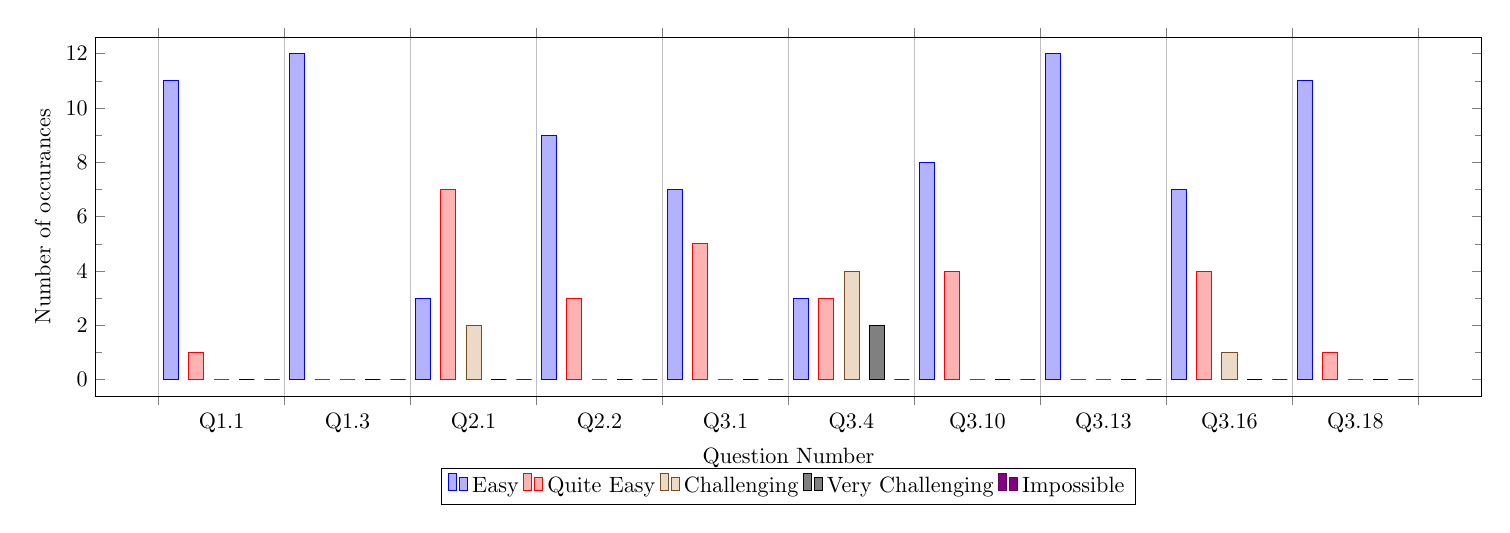
\begin{tikzpicture}[scale=0.8]
\begin{axis}[ybar interval, ymax=12, minor y tick num = 1, legend style={at={(0.5,-0.2)}, anchor=north,legend columns=-1}, bar width= 0.1cm, x=2cm, 	enlargelimits=0.05, ybar interval=0.6, xlabel= Question Number, ylabel= Number of occurances,symbolic x coords={Q1.1, Q1.3, Q2.1, Q2.2, Q3.1, Q3.4, Q3.10, Q3.13, Q3.16, Q3.18, None},xtick=data]


\addplot coordinates { (Q1.1, 11) (Q1.3,12) (Q2.1, 3) (Q2.2, 9) (Q3.1, 7) (Q3.4, 3) (Q3.10, 8) (Q3.13, 12) (Q3.16, 7) (Q3.18, 11) (None, 10)};

\addplot coordinates { (Q1.1, 1) (Q1.3,0) (Q2.1, 7) (Q2.2, 3) (Q3.1, 5) (Q3.4, 3) (Q3.10, 4) (Q3.13, 0) (Q3.16, 4) (Q3.18, 1) (None, 10)};

\addplot coordinates { (Q1.1, 0) (Q1.3,0) (Q2.1, 2) (Q2.2, 0) (Q3.1, 0) (Q3.4, 4) (Q3.10, 0) (Q3.13, 0) (Q3.16, 1) (Q3.18, 0) (None, 10)};

\addplot coordinates { (Q1.1, 0) (Q1.3,0) (Q2.1, 0) (Q2.2, 0) (Q3.1, 0) (Q3.4, 2) (Q3.10, 0) (Q3.13, 0) (Q3.16, 0) (Q3.18, 0)  (None, 0)};

\addplot coordinates { (Q1.1, 0) (Q1.3,0) (Q2.1, 0) (Q2.2, 0) (Q3.1, 0) (Q3.4, 0) (Q3.10, 0) (Q3.13, 0) (Q3.16, 0) (Q3.18, 0) (None, 0)};



\legend{Easy, Quite Easy, Challenging, Very Challenging, Impossible}
\end{axis}
\end{tikzpicture}
\end{figure}

%Overall easiness% 
The first thing that can be noticed is that overall the participants found the lab marking system  fairly easy to use and understand. The two tasks that users found the hardest to do were mark students and create labs, which are the most complex part of the lab marking system. It would be expected that first time users of the system would find these difficult to understand at first. Though it can be seen with the "update student mark" task that  once the participants have marked one student they now found it much easier to mark students. 

%Difficulty of creating labs%
\noindent It can be seen thanks to graph shown in figure(\ref{graph:results}) that many users found the creating of new labs to be a difficult task to complete. While watching participants  I noticed that many of them were confused on how questions were added to labs.\\ 

%Simplicity of student section%
\noindent Question 1.1 tasked participants to sign in as a student and see what mark they were given. As the results of both the table(\ref{table:usability}) and the graph(\ref{graph:results}) all participants found this to be easy to do. This is great to see, as the lab marking system is meant to make it easier for students to find out their marks and this task has shown that process for a student finding their marks is very straight forward.


\subsubsection*{Yes/No Question}
Three of the questions in the usability study were yes and no questions. These questions were designed to see if users understood key parts of the lab marking system.

\subsubsection*{Q2.3: Student Button Colours}

\begin{wrapfigure}[7]{r}{0.5\textwidth}
\vspace*{-\baselineskip}
\begin{figure}[H]
\caption{Q2.3: Know what the different student colours mean?}

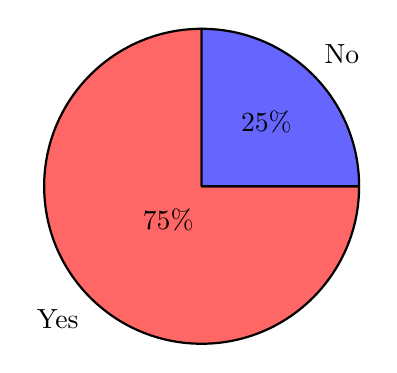
\begin{tikzpicture}
    \pie[rotate=90,radius =2, color={red!60, blue!60}]{75/Yes, 25/No}
\end{tikzpicture}

\end{figure}
\end{wrapfigure}

The first question was to check if participants understood what the different coloured buttons for students represented and 75\% did understand what they represented. The fact that 25\% of the participants did not understand what the legend shows and the colours to which they correlate should be improved.




\subsubsection*{Q3.6: Visibility Button}

\begin{wrapfigure}[7]{l}{0.5\textwidth}
\vspace*{-\baselineskip}
\begin{figure}[H]
\caption{Q3.6 Know what visible / not visible means?}

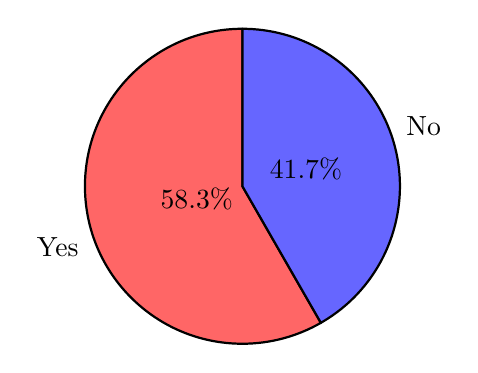
\begin{tikzpicture} 
    \pie[rotate=90,radius = 2, color={red!60, blue!60}]{58.3/Yes, 41.7/No}
\end{tikzpicture}

\end{figure}
\end{wrapfigure}

The second yes/no question was to do with the creation of new labs and the understanding of what the visible / not visible button did to individual questions. Only 58.3\% of participants understood what this button meant. Since this is a key piece of functionality and allows lecturers to control what questions students can see in their result, it must be improved. Many participants suggested the inclusion of tool tips to help understand what the button was meant to do. 


\subsubsection*{Q3.8 Creation Alerts}



The final yes/no question delete with the error handling of the lab creation page. Participants were asked to create a lab that was not complete and attempt to submit it. They were then

\begin{wrapfigure}[7]{r}{0.5\textwidth}
\vspace*{-\baselineskip}
\begin{figure}[H]
\caption{Q3.8: Did an alert appear}

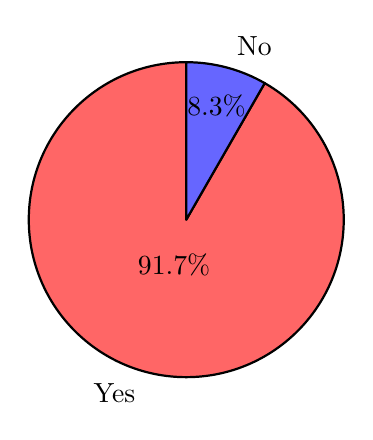
\begin{tikzpicture}
    \pie[rotate=90,radius =2, color={red!60, blue!60}]{91.7/Yes, 8.3/No}
\end{tikzpicture}

\end{figure}
\end{wrapfigure}

\noindent asked to note if an alert appeared informing of an incomplete lab. It was expected that this question would have a 100\% yes response, however one participant managed to find a combination of inputs that was not complete but did submit. The participant in question provided how he got this outcome and I fixed the error detection to prevent it from occurring again.


\subsubsection{Qualitative Questions}

As part of each of the task participants were asked to provide feedback about the task and any improvements that could be made to each of the different parts of the lab marking system. These qualitative questions allowed participants to provided useful feedback and improvements that could be done. The summarised feedback will be broken down into the four main pages: Results, Marking, Lab Creation and Lab Manager.

\subsubsection*{Results Page}

The qualitative questions relating to results page come from both the student section and lecturers as they are both based on a similar design. The overall design of the two results pages was liked by the participants and many stated that they "liked the transition when you drop down the box". Though some participants did not immediately understand that labs were click-able and suggested that on hovering over the lab that "the mouse should change to a hand"  to show that it is click-able. What was noticeable from the feed back was that users were having a hard time reading the text inside the result tables. Many participants suggested "increasing the fonts" or "make the font bold". This is easily done by adjusting the CSS responsible for the font size. 

\noindent Now the feedback that solely relates to the student version of the results page. There was little unique feedback for the student version since it has a very simplistic design. The only feed back that was given what that there was "No indication of drop-down menu until clicked on" this applied to labs where the student had not been marked yet and was meant to discourage users from clicking those labs.

\noindent Finally the feed back about the lecturers version of the results page. Overall feedback showed that users found it "Easy to find student and view marks", though many participants had suggestions for improving the results pages. The largest comment was "A search bar to search to shorten the student list" this would be useful to have as we have upwards of 160 student and scrolling though 160 names looking for one specific name would be challenging and reduce the systems overall usability. Multiple participants also stated that "clicking on the marks closed the lab", I had not thought that users would be clicking the marks but one participant stated that they would not be able to highlight and copy marks as they cannot click on it. So this should be corrected for the next version.



\subsubsection*{Lab Marking Page}

The lab-helper section was where participants were asked to test out the marking functionality of the lab marking system. The task to mark students had the second highest difficulty of any task and therefor has a large amount of feedback about parts they did not understand and how to make certain sections easier to understand. 

The first things participants were saying was "make it more obvious where the marking section is", I noticed that quite a few participants did not notice the "mark lab" button in the navigation bar. Some where even suggested that lab-helpers should be "directed to the marking page when they logged in" and not to the results page. Both of these issues could be sorted by the inclusion of a button in the results page that takes the user to the lab marking page. It easier to navigate too and allows users a quick way to access it when they login. 

Something multiple participants raised was "confusion of the student colour coding" as they they did not know the difference between fully marked and just normal marked. It was suggested that the use of tool tips on the on the colour code legend would be useful to explain the different colours. 

The most common issue stated was that "Initially they did not know they could click the yes/no buttons" this was in reference to the boolean type questions where you could click the button to swap between yes and no. In addition to this participants did not know if they were setting student mark to no as it was quite ambiguous. Some participants suggested some solutions to the issues which were the use of a "tick box or a drop down selection" instead of the button, both of these options would make it easier to tell which option has been selected and know that they can interact with it.

Some participants found the marking of students to become easier once they had an I of how it functions stating "Once you learn how to use it the system is very smooth to use". This shows that while the marking of students has an initial learning curve as with many system, once users have time to practise with it they can use it without many problems.

While the marking of students has does have a few issue that need to be sorted, participants did not find any issues that severely impacted the usability and functionality of the lab marking system.



\subsubsection*{Lab Creation Page}

The feedback from participants showed that they found the creation of labs to be the most challenging aspect of the lab marking system. The complexity of making labs resulted in a large amount comments on how to improve the design to make it more intuitive to use. Most of the issues raised by participants were the same, showing that these issues have a major impact on the marking of labs. 

Participants provided a lot of comments about the selection of question types. Many felt that the buttons to select question types "are not obvious", as it is not clear what the buttons in the side bar are meant to do. Some participants also stated that they did not know what "the different types of questions do" and suggested the use of on hover tool-tips to give an explanation of what each question type is.

When it came to the question tiles participants also had issues and suggested improvements. The most immediate issue participants thought "the question tiles were pop-ups" and from personal observation tried to submit labs them thinking that they would then select the next question. This issue will need to be solved to make the creation of labs more usable, the rewording of question adding buttons will probably help but the most important would be the redesign of question tiles to look more interlocking and not look less like a pop-up

The fact that participant had issues which severely  impact on the usability of the lab creation page shows that it needs major improvements. Participants did say that "they could create labs once it was explained to them" therefor showing that the lab creation page does fill the requirement it needs too, but the learning curve for using it needs to be reduced



\subsubsection*{Lab Manager Page}

Participants did not raise any issues with the lab management page feeling that all the functionality "worked very well and was easy to preform", although they did provided some suggestion to help make the lab manager better. A few suggested that the "lab management page should be the home page for lecturers", I can understand this idea as a lot of the functionality for lecturers is based on this page and would make it quicker for lecturers preform actions. One participant suggest the inclusion of "a pop-up to states where a lab has been exported to" this would be useful in helping lecturers find labs quickly that they have exported. Final thing that was suggested was that it should be possible to "export the total mark for a course", this would make it easy to compare the whole courses results in a spread sheet form.



\subsection{Implementation Of Feedback}

Using the feedback obtained through the usability case study I  have implemented a few changes to the design of the lab marking system. This is to help improve the overall usefulness of the system and make certain parts of the system easier to understand and interact with. The improvements done to the system are listed below with description and comparison showing the lab marking system before and after the changes.  


\subsection{Evaluate Requirements}

In addition to the usability case study, to evaluate the lab marking system I must check how successful the project was at implementing the requirements of a digital lab marking system. 

To evaluate if the project matches the requirements of the digital lab marking system, the functional requirements originally shown in section \ref{sec:requirements} have been repeated here. Though this time each requirement has been highlighted according to its implementations. The colour code is: Green means the requirement was implemented in the project, Yellow means that the requirement was not implemented but not guaranteed to be and finally Red is for requirements that were promised but did not get implemented.   



\begin{spacing}{1.1}
\begin{longtable}{|p{0.09\linewidth}|p{0.6\linewidth}|p{0.1\linewidth}|
p{0.1\linewidth}|}
\caption{Functional Requirements} \label{table:eval-funct-user} \\ \hline
\textbf{ID} & \textbf{Requirement} & \textbf{Access} & \textbf{Priority}\\
\hline \hline

\rowcolor{Green} \rid{FR} &  Login to view system & 1,2,3,4 & Must\\ \hline
\rowcolor{Green} \rid{FR} &  Accounts created for them & 1,2,3,4 & Must\\ \hline
\rowcolor{Red} \rid{FR} &  Change password & 1,2,3,4 & Must\\ \hline
\rowcolor{Green} \rid{FR} &  Logout & 1,2,3,4 & Must \\ \hline
\rowcolor{Yellow} \rid{FR} &  Login using university ID & 1,2,3,4 & Could\\ \hline

\rowcolor{Green} \rid{FR} &  Remove students from courses & 1, 2 & Must\\ \hline
\rowcolor{Yellow} \rid{FR} &  Update student accounts & 1,3 & Could \\ \hline

\rowcolor{Green} \rid{FR} &  Look up students in lab & 2,3 & Must\\ \hline
\rowcolor{Green} \rid{FR} &  Select students from lab list & 2,3 & Must\\ \hline
\rowcolor{Green} \rid{FR} &  Leave comments about students & 2,3 & Must\\ \hline
\rowcolor{Green} \rid{SR} &  Save marks & 2,3 & Must\\ \hline
\rowcolor{Green} \rid{SR} &  Update marks & 2,3 & Must\\ \hline
\rowcolor{Red} \rid{SR} &  Delete marks & 2,3 & Must\\ \hline
\rowcolor{Green} \rid{FR} &  Search for student by name & 2,3 & Should\\ \hline
\rowcolor{Yellow} \rid{FR} &  Mark student even if they are not in the system & 2,3 & Could \\ \hline

\rowcolor{Green} \rid{FR} &  Assign students to courses & 1 & Should\\ \hline
\rowcolor{Green} \rid{FR} &  Assign lectures to courses & 1 & Should\\ \hline

\rowcolor{Green} \rid{FR} &  Create marking schemes & 2 & Must\\ \hline
\rowcolor{Green} \rid{FR} &  Display generated stats & 2 & Must\\ \hline
\rowcolor{Green} \rid{FR} &  See submitted marks & 2 & Must\\ \hline
\rowcolor{Yellow} \rid{FR} &  Generate end of year spread sheets & 2 & Should\\ \hline
\rowcolor{Green} \rid{FR} &  Editing of students in class & 2 & Should\\ \hline
\rowcolor{Green} \rid{FR} &  Look at students stats & 2 & Should\\ \hline
\rowcolor{Green} \rid{FR} &  Update marking scheme & 2 & Should \\ \hline
\rowcolor{Green} \rid{FR} &  Delete marking schemes & 2 & Should\\ \hline
\rowcolor{Yellow} \rid{FR} &  Able to assign students to set labs & 2 & Could \\ \hline
\rowcolor{Yellow} \rid{FR} &  Set penalties for late marking & 2 & Could \\ \hline
\rowcolor{Green} \rid{FR} &  Able to export to vision & 2 & Could\\ \hline
\rowcolor{Green} \rid{FR} &  Set what parts of the marking scheme students can see & 2 & Could\\ \hline
\rowcolor{Yellow} \rid{FR} &  Create peer marking scheme & 2 & Could\\ \hline

\rowcolor{Green} \rid{FR} &  Access Marking Scheme & 3 & Must\\ \hline
\rowcolor{Green} \rid{FR} &  Enter selected students mark & 3 & Must\\ \hline
\rowcolor{Green} \rid{FR} &  Submit student mark & 3 & Must\\ \hline
\rowcolor{Green} \rid{FR} &  Select the lab they are helping in & 3 & Must\\ \hline

\rowcolor{Green} \rid{FR} &  See current mark & 4 & Must\\ \hline

\rowcolor{Green} \rid{FR} & Show different displays depending on access level & & Must\\ \hline
\rowcolor{Green} \rid{FR} & Load students current lab mark scheme & & Must\\ \hline
\rowcolor{Yellow} \rid{FR} & Apply penalty for late lab completion & & Could\\ \hline
\rowcolor{Green} \rid{FR} & Create a set of useful stats based on lab & & Must\\ \hline
\rowcolor{Green} \rid{FR} & Store what class student belong too & & Must\\ \hline
\rowcolor{Green} \rid{FR} & List of all students in class & & Must\\ \hline

\end{longtable}
\end{spacing}
\setcounter{requirement}{1}

The table of requirements makes it easier to tell how many of the requirements the project meets. This projects covers 75\% of the requirements, having implemented 31 of the 41 possible requirements for a lab marking system. This leaves only ten non-implemented requirements and of those ten only two of them were 'must' requirements, one of them was a 'should' and the remaining seven were 'coulds'.

\subsubsection*{Miniumum Requirements}

The fact that only twenty-two out of the twenty-four (91\%) of the  must requirements were  implemented shows that the developed lab marking system does meet the minimum requirements of the system. The two requirements that the system did not meet are the ability for users to change their password and the ability to delete marks.

As this project was meant to provide a prototype version of digital lab marking system whose focus was on being able to create a mark labs. The inability of users to update their passwords is not a major issue, firstly because when accounts are created random passwords are generated meaning there is some security for accounts and secondly if the marking system was to be integrated with existing university accounts users would already have a way to change their password.

The inability to delete marks is a more major issue, though during development I did not see any reason on why a mark would need to be deleted. Currently the only way to delete a mark completely from the database is to remove a student from a course and then add them back on to it. This has its own issues in that it is time consuming to do and deletes all the lab marks for the student not just a specific one. A mark can also be updated to its default which would be the equivilant of the mark being deleted.

\subsubsection*{Could and Should}

At the start of the project I stated that there would be as many "could" and "should" requirements implemented as possible. There were 17 should/could functional requirement of these 17 only 9 (52.9\%) were implement. Of these nine requirements only one of them was a "should" and that was to "Generate end of year spread sheets" which is doable thanks to the "IO" class which can output spread sheets. All that is needed is the data to put into it and that can be recovered using a mysqli query.    

The other eight requirements that were not included were "could" priority requirements which are the first requirement to be abandoned if time does not allow. So it is not surprising that the largest number of none implemented requirements are "could" requirements, these are requirements that can be implemented in a later version and there absence from the lab marking system does not have a large effect on its overall usability and functionality.


\subsection{Aim and Objective}

In addition to evaluating the project on how successful it was at meeting the requirements for a lab marking system, it can also be evaluated on how successful it was at reaching its aim and its multiple objectives.

Firstly we must start with the objective of this project which was to "implement  a  system  for  the  digital  marking  and analysis of computer labs and to help improve the speed at which they are marked". This project was successful in designing and implementing a digital lab marking system. However to assess if the system has enhanced the speed of the process of marking a more thorough study would require to be run. Though it can be seen that the time between marking a student's work and them viewing their marks has become nigh on instantaneous.

Now for the objectives: this project has seven objectives it set out to complete. Firstly "Simplify the way that lab marks are currently processed" the developed system does this by allowing marks to be instantly seen by lecturers and students, removing the time it took for lab-helpers to hand in marking  sheets and for the lecturer to transfer the marks to a spread sheet.

The second aim was "Allow lecturers to create marking schemes on-line that lab-helpers can access": this aim is met in the lab creation page where lecturers can create new labs and the lab marking page where the labs can be accessed.

The third and fourth aims are "Lab helpers can mark students using the marking schemes" and "Lab Helpers are able to mark labs using an on-line system". Both of these aims are successfully met by the lab marking page, lab helpers can select students and mark them and even update current marks and since the lab marking system is a web application lab helpers can do this on-line.

The fifth aim was to "Allow students to see the mark they achieved from the lab instantly", this is done automatically by the system meaning the moment that a student has been marked they can go to their results page and see their results for the lab.

The sixth aim was to "Provide useful statistics and graphs for lecturers and students". The lab marking system does provide statistics for both students and lecturers, but does not provide a graphical representation of these stats and is something that should be added in a later version. Additionally lecturers could be given a wider variety of statistics as they only have stats on a lab by lab basis not statistics for the whole course.

The seventh and final aim was to "Provide different views for student, lab helpers and lecturers", this is done in both the results page and lab marking page. On the results page students are given a different layout compared to lecturers- they can only see their own results while lecturers are able to select students whose results they wish to view. While on the marking page lecturers are able to select from any labs on a course while lab helpers can only see and select labs that the lecturer has declared are mark-able.



\subsection{Overall Evaluation}

Overall the evaluation of the system shows it to be a good implementation of a digital marking system. The usability case study showed that users found it easy to understand and quickly picked up how to use it, while also helping to point out improvements that could be make to the system. The system also met a majority of the requirements needed in a digital marking system, thus showing it has the functionality required to be a useful system. Finally the lab marking system as a whole meets the aim and objective of this projects, showing that development of it was a success.

It however needs some improvements, especially the lab creation section which was shown to be a little complex to understand and use. Additionally search bars can be added to areas where there is a need to select students, to help make it easy to find students in large classes. Finally the addition of more statistics would greatly improve the usefulness of the system for lecturers and students.







%%%%%%%%%%%%%%%%%%%%%%%%%%%%%%%%%%%%%%%%%
%										%
%     	       Discussion				%
%										%
%%%%%%%%%%%%%%%%%%%%%%%%%%%%%%%%%%%%%%%%%
\newpage
\section{Discussion}

This section is for discussion of the digital lab marking system as a whole. It includes discussion about the overall development of the system, limitations that currently exist in the lab marking system, improvements that can be implemented later and a conclusion which covers all the different parts of the project.

\subsection{Development}

\subsubsection{Issues}

Originally I had be planning to develop the lab marking system using cakePHP,but as I did more research I quickly found out that it would take more time to setup my computer at home and at the university than the framework would help me save. I therefore decided  not to use it and just have no PHP framework when developing the system.

In addition to not using cakePHP I did not manage to use d3 to provide graphical representations of statistics. This was because when I started trying to implement d3 I discovered that it was naturally dynamically responsive, this meant that any change in the screen size would result in elements moving expectantly and give the website a bad appearance. There is a way to make d3 graphs responsive but given the amount graphs this would add to the lab marking system I decided instead to focus my time on more important functionality. 



\subsection{Limitations}

The aim of this project is to enable lecturers to mark students using a digital marking system. This project was successful in creating this marking system, but it has limitations on what it is able to do. These limitations are all discussed here, along with how to solve them or mitigate the effect they have on the system as a whole.

\subsubsection{Only Three Question Types}

The current version of the lab marking system only allows lecturers to create lab questions of three different types, these being : scale questions, Boolean questions and text questions. This lack of question variety can be seen as a limitation of the system, though I have designed the system so that it is easy to create new types of questions.

\subsubsection{Student Only Lab Helpers}




\subsection{Future Improvements}
The digital lab marking system has many improvements that can be implemented; some of these are requirements that I was not able to implement in the time available. Other improvements for the system came from feedback obtained from the usability case study. 

With more time d3 could be converted to be dynamically responsive and make it possible to generate graphs for the statistics being generated.

\subsubsection{Peer Marking}

Adding to the ability to do peer marking using the lab marking system would make it more useful.

\subsubsection{Comparing Students}

It was suggested by a few of the participants of the usability case study that lecturers should be able to select multiple students and see their marks.

\subsubsection{Track Who Marked What Student}

One of the original requirements which was then brought up again during the usability case study, was the ability to track who lab-helpers were marking. This is to make it easy to find out who marked a student if an issue arises, and helps lecturers analyse the quality of a lab-helper's marking. 
I was unable to implement this functionality into the lab marking system due to time constraints and the need to redesign part of the database to store the markers details. I feel that it would provide a very useful tool for lecturers and should be implemented in the next version.


\subsection{Conclusion}

In conclusion this project to develop a digital lab marking system has provided a variety of challenges.

Overall I would state that this project was successful in developing a digital system for the marking of labs. It has a few flaws at the moment but nothing that cannot not be sorted out in the next version of the system.









%%%%%%%%%%%%%%%%%%%%%%%%%%%%%%%%%%%%%%%%%
%										%
%     		Bibliography				%
%										%
%%%%%%%%%%%%%%%%%%%%%%%%%%%%%%%%%%%%%%%%%


\newpage
\printbibliography[heading=bibintoc]
\let\cleardoublepage\clearpage


%%%%%%%%%%%%%%%%%%%%%%%%%%%%%%%%%%%%%%%%%
%										%
%     		Appendices					%
%										%
%%%%%%%%%%%%%%%%%%%%%%%%%%%%%%%%%%%%%%%%%

\newpage
\begin{appendices}

\let\cleardoublepage\clearpage

% \chapter{Useability Case Study}
% \includepdf[pages={1}]{pdf/UseabilityCaseStudy.pdf}
% \section{Useability Case Study}
% \includepdf[scale=0.85, pages=-]{pdf/UseabilityCaseStudy.pdf}


%Requirements Analysis Document
% \includepdf[scale=0.9,clip,trim=0cm 0cm 0cm 2cm,pages={1},pagecommand={\section{Requirements Questionaire} \label{app:requirements}}]{pdf/RequirementsQuestionaire.pdf} 
% \includepdf[scale=0.9,clip,trim=0cm 0cm 0cm 2cm,pages={2-6},pagecommand={}]{pdf/RequirementsQuestionaire.pdf}


%Useability Case Study Document
% \includepdf[scale=0.9,clip,trim=0cm 0cm 0cm 2cm,pages={1},pagecommand={\section{Useability Case Study Questionaire} \label{app:ucs}}]{pdf/UseabilityCaseStudy.pdf} 
% \includepdf[scale=0.9,clip,trim=0cm 0cm 0cm 2cm,pages={2-8},pagecommand={}]{pdf/UseabilityCaseStudy.pdf}


\end{appendices}
\end{document}